\newpage
\section{Auswertung}
    \subsection{Vorbereitungsmessungen}
        Für die erste Vorbereitungsmessung werden beispielhaft die Messungen für einen Zylinder, einer Reihe aus vier Zylindern und einer Reihe aus acht Zylindern der Länge \SI{50}{\milli\metre} mit den 
        entsprechenden Oszilloskopmessungen verglichen. Die Abbildungen~\ref{fig:pre_vgl} zeigen, dass die Messungen per Computersoftware und Oszilloskop weitgehend übereinstimmen. Die Peaks und deren 
        relativen Höhen auf dem Oszilloskop spiegeln die Darstellung der Computersoftware wieder, werden jedoch weniger scharf dargestellt. Deswegen ist es sinvoll die Computermessungen zur weiteren Analyse
        zu nutzen. 
        \begin{figure}
            \centering
            \begin{subfigure}[b]{0.45\textwidth}
                \centering
                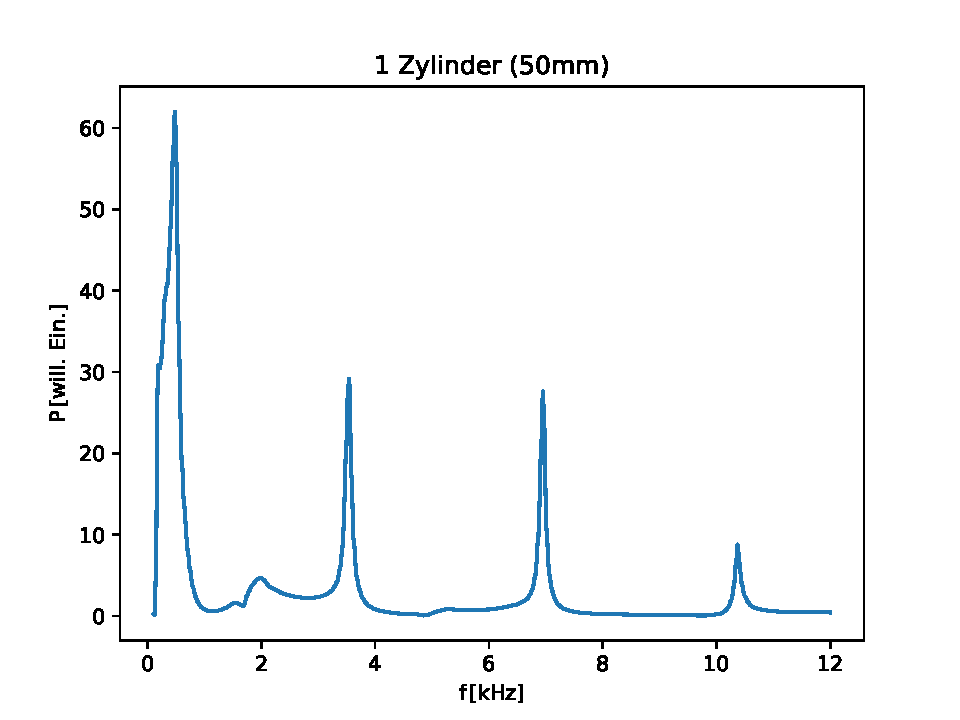
\includegraphics[scale=0.4]{./pictures/1_Zylinder_50mm.pdf}
                \caption{In der Abbildung ist die Einhüllende, sowie das schwingende elektrische Feld eines linear gechirpten Laserpulses zu sehen.}
                \label{fig:e_feld_chirp}
            \end{subfigure}
            \hfill
            \centering
            \begin{subfigure}[b]{0.45\textwidth}
                \centering
                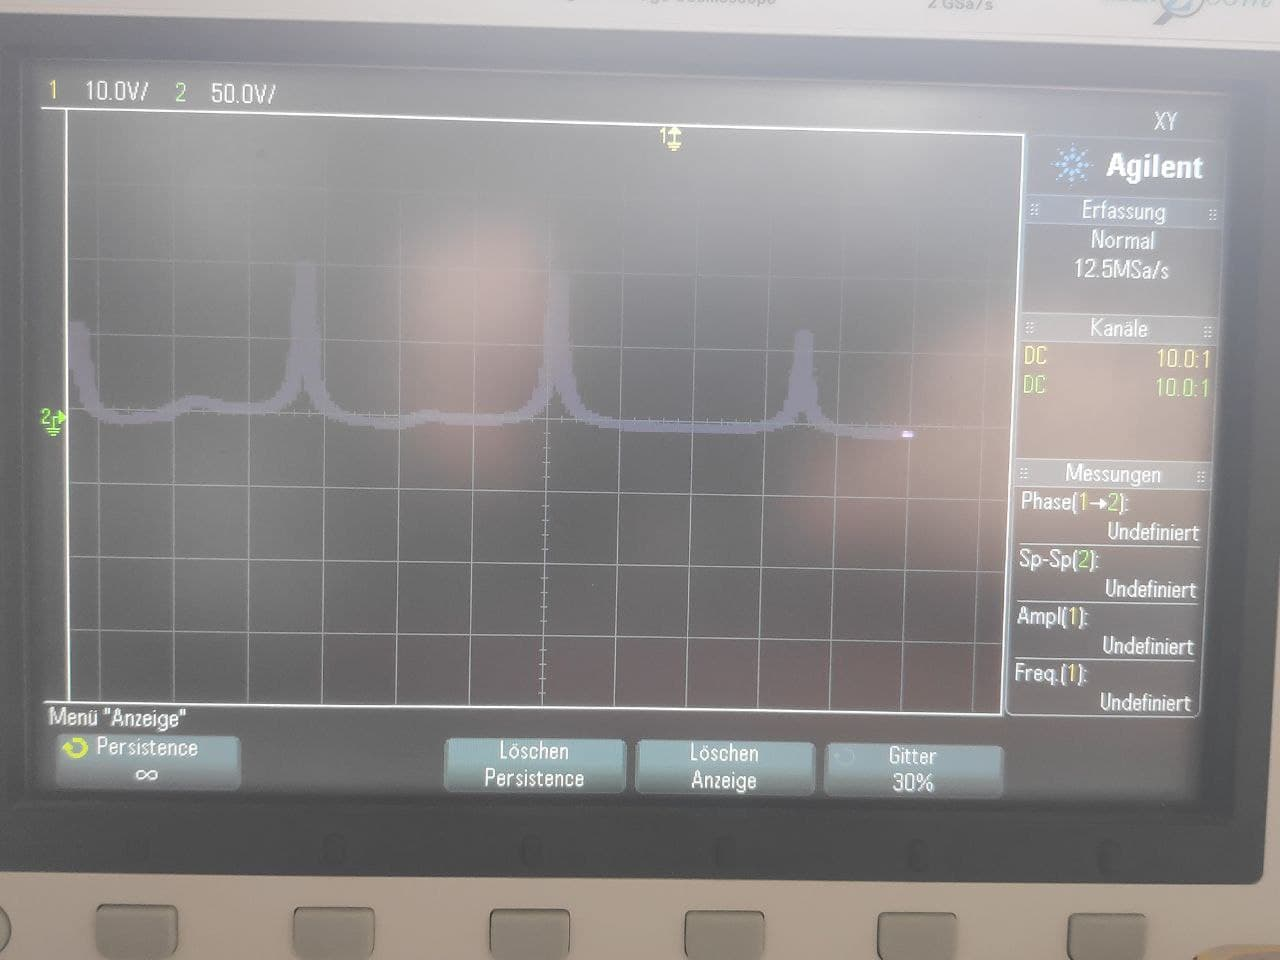
\includegraphics[scale=0.13]{./pictures/1_Zylinder.jpg}
                \caption{In der Grafik wird der Chirp des Pulses als Änderung der Kreisfrequenz über den zeitlichen Verlauf des Pulses verdeutlicht.}
                \label{fig:chirp}
            \end{subfigure}

            \centering
            \begin{subfigure}[b]{0.45\textwidth}
                \centering
                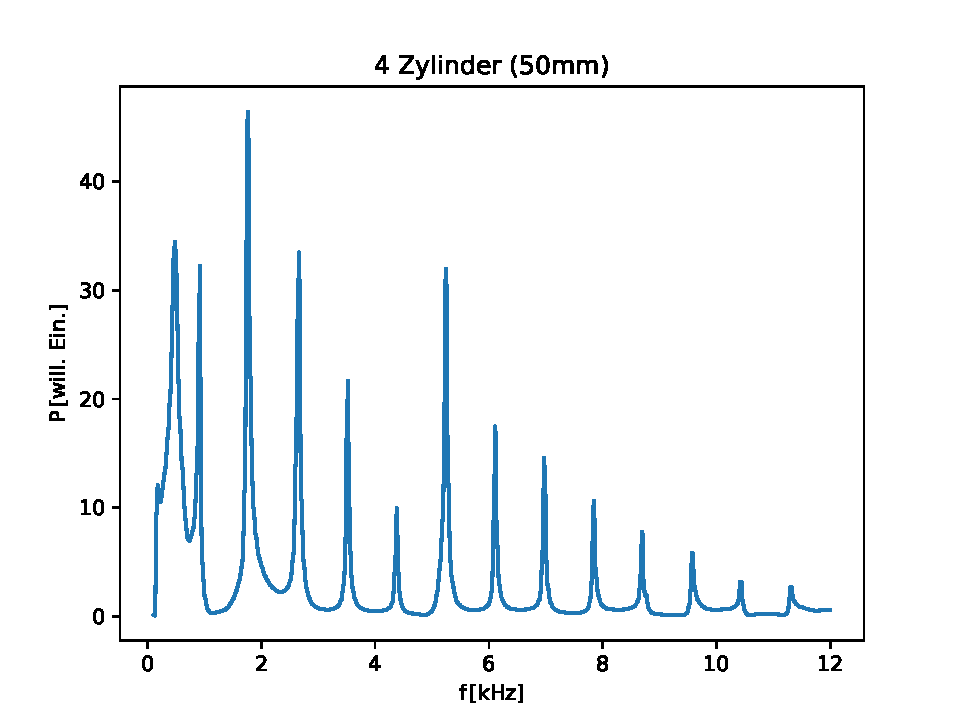
\includegraphics[scale=0.4]{./pictures/4_Zylinder_50mm.pdf}
                \caption{In der Abbildung ist die Einhüllende, sowie das schwingende elektrische Feld eines linear gechirpten Laserpulses zu sehen.}
                \label{fig:e_feld_chirp}
            \end{subfigure}
            \hfill
            \centering
            \begin{subfigure}[b]{0.45\textwidth}
                \centering
                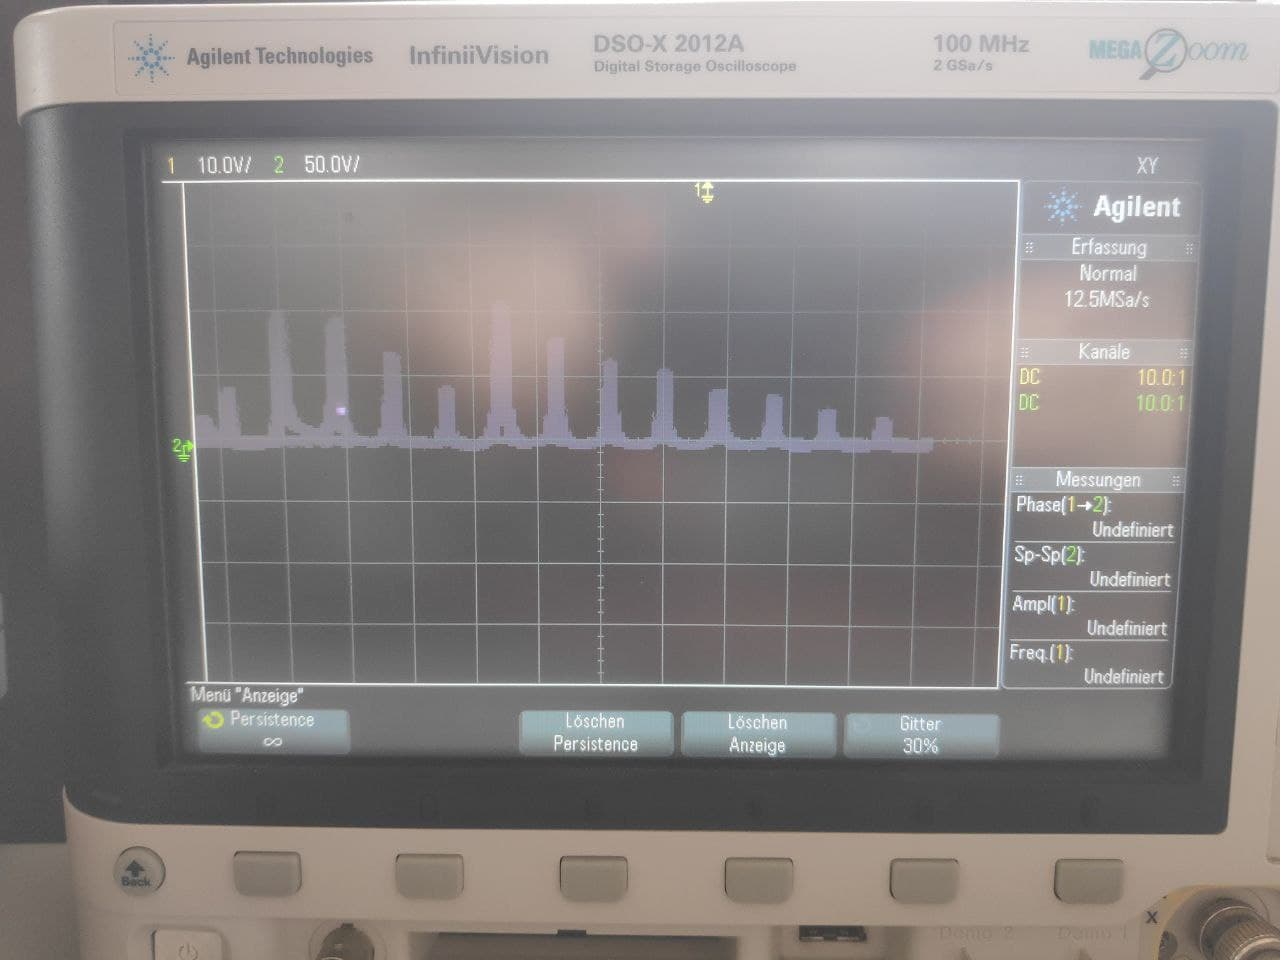
\includegraphics[scale=0.13]{./pictures/4_Zylinder.jpg}
                \caption{In der Grafik wird der Chirp des Pulses als Änderung der Kreisfrequenz über den zeitlichen Verlauf des Pulses verdeutlicht.}
                \label{fig:chirp}
            \end{subfigure}

            \centering
            \begin{subfigure}[b]{0.45\textwidth}
                \centering
                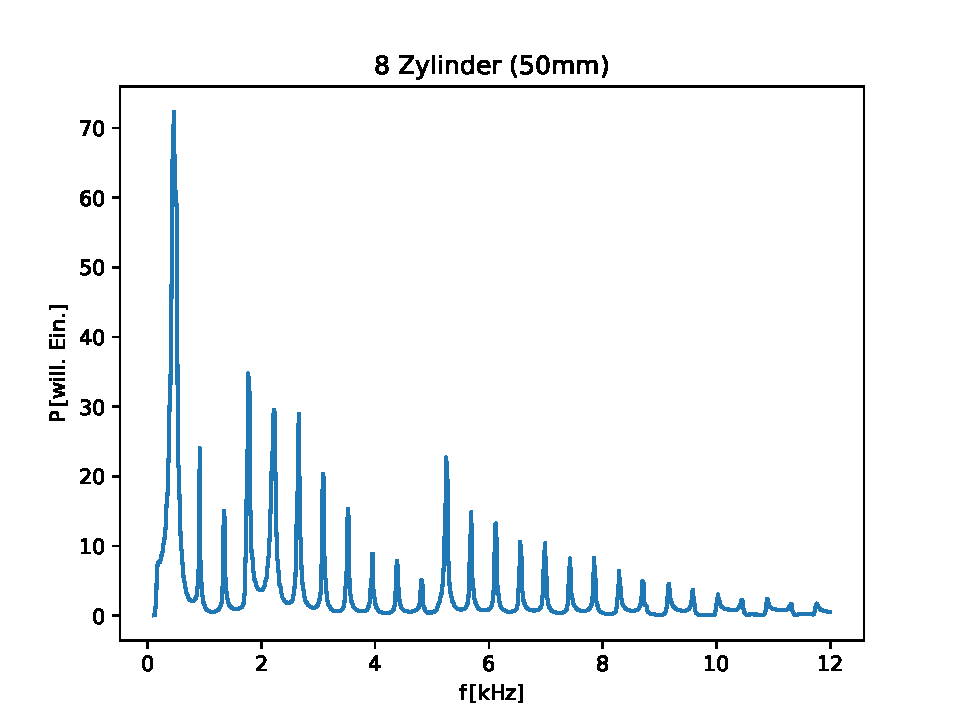
\includegraphics[scale=0.4]{./pictures/8_Zylinder_50mm.pdf}
                \caption{In der Abbildung ist die Einhüllende, sowie das schwingende elektrische Feld eines linear gechirpten Laserpulses zu sehen.}
                \label{fig:e_feld_chirp}
            \end{subfigure}
            \hfill
            \centering
            \begin{subfigure}[b]{0.45\textwidth}
                \centering
                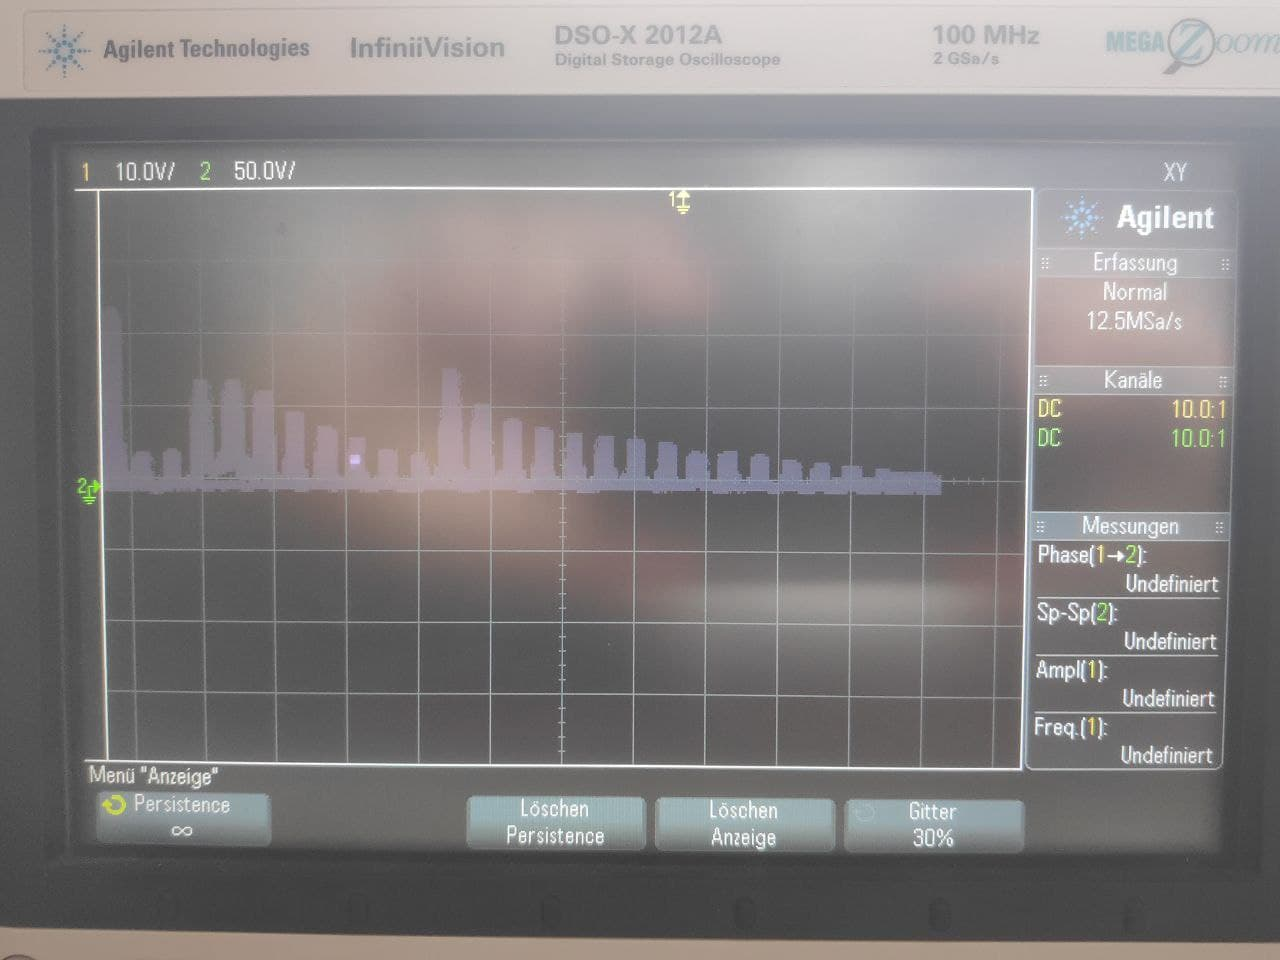
\includegraphics[scale=0.13]{./pictures/8_Zylinder.jpg}
                \caption{In der Grafik wird der Chirp des Pulses als Änderung der Kreisfrequenz über den zeitlichen Verlauf des Pulses verdeutlicht.}
                \label{fig:chirp}
            \end{subfigure}
            \caption{sd}
            \label{fig:pre_vgl}
        \end{figure}
    \FloatBarrier

    \subsection{Wasserstoffatom}
        \subsubsection*{Resonanzfrequenzen bei $\alpha$=180°}
            Zunächst wird das gemessene hochaufgelöste Frequenzspektrum des Hohlraumresonators bei einem Winkel von $\alpha=\SI{180}{\degree}$ in Abbildung \ref{fig:hatom_180} dargestellt.
            \begin{figure}
                \centering
                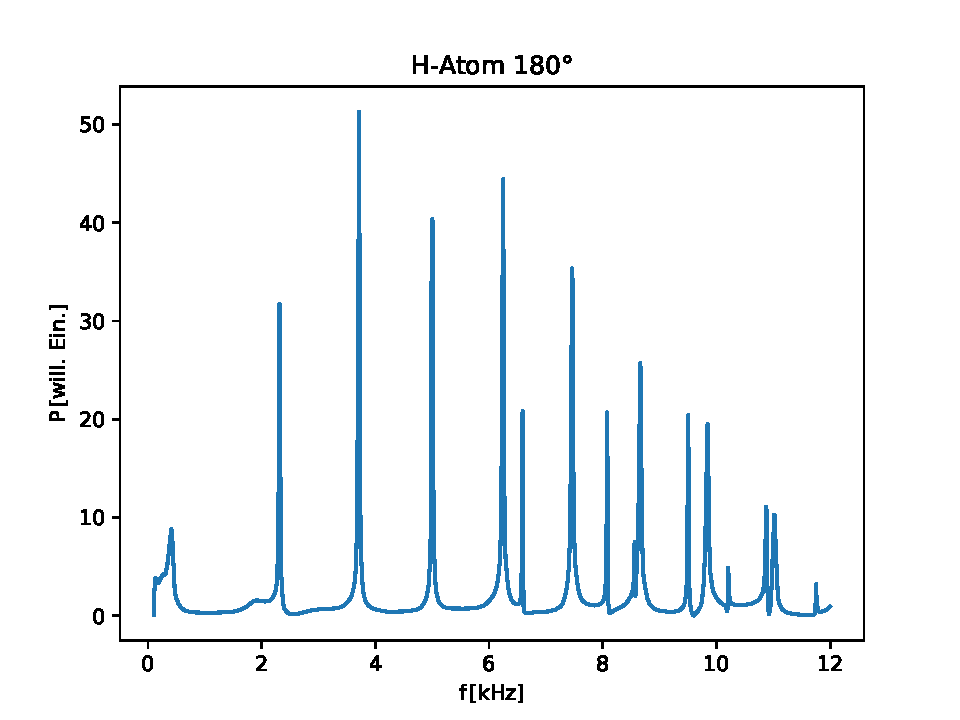
\includegraphics[scale=0.7]{./pictures/hatom_180.pdf}
                \caption{In der Abbildung ist die Einhüllende, sowie das schwingende elektrische Feld eines linear gechirpten Laserpulses zu sehen.}
                \label{fig:hatom_180}
            \end{figure}

            \FloatBarrier
            Mit Hilfe des Oszilloskops werden die in Abbildung \ref{fig:hatom_180} zu sehenden Resonanzfrequenzen analysiert und ihre Ordnung, Amplitude und Phasenverschiebung in Tabelle~\ref{tab:phasenverschiebung} 
            aufgelistet.
            \FloatBarrier
        \newpage
        \subsubsection*{Winkelabhängigkeit gewählter Resonanzfrequenzen}
            Die Druckamplitude der Resonanzfrequenzen wird für die Resonanzfrequenzen \SI{2.3}{\kilo\hertz}, \SI{2.3}{\kilo\hertz}, \SI{2.3}{\kilo\hertz} und \SI{2.3}{\kilo\hertz} in Abhängigkeit des Winkels
            $\alpha$ aufgetragen. Die in den Abbildungen \ref{fig:H_atom_resonanz_1_2310Hz} und \ref{fig:H_atom_resonanz_3_4999Hz} zu sehende Druckamplitudenverteilungen scheinen einem Halbkreis zu entsprechen. 
            Dies deutet darauf hin, dass es sich um Äquivalente eines 1s$_0$-Orbitals handelt. Die in Abbildung \ref{fig:H_atom_resonanz_2_3711Hz} zu sehende Druckamplitudenverteilungen weißt auf ein 
            2p$_0$-Orbital hin. In Abbildung \ref{fig:H_atom_resonanz_4_7470Hz} scheint das Äquivalent eines 4f$_0$-Orbitals aufgenommen worden zu sein, dessen Keule im niedrigen Winkelbereich abgeschnitten 
            ist.
            \FloatBarrier
            \begin{figure}[ht]
                \centering
                \begin{subfigure}[b]{0.45\textwidth}
                    \centering
                    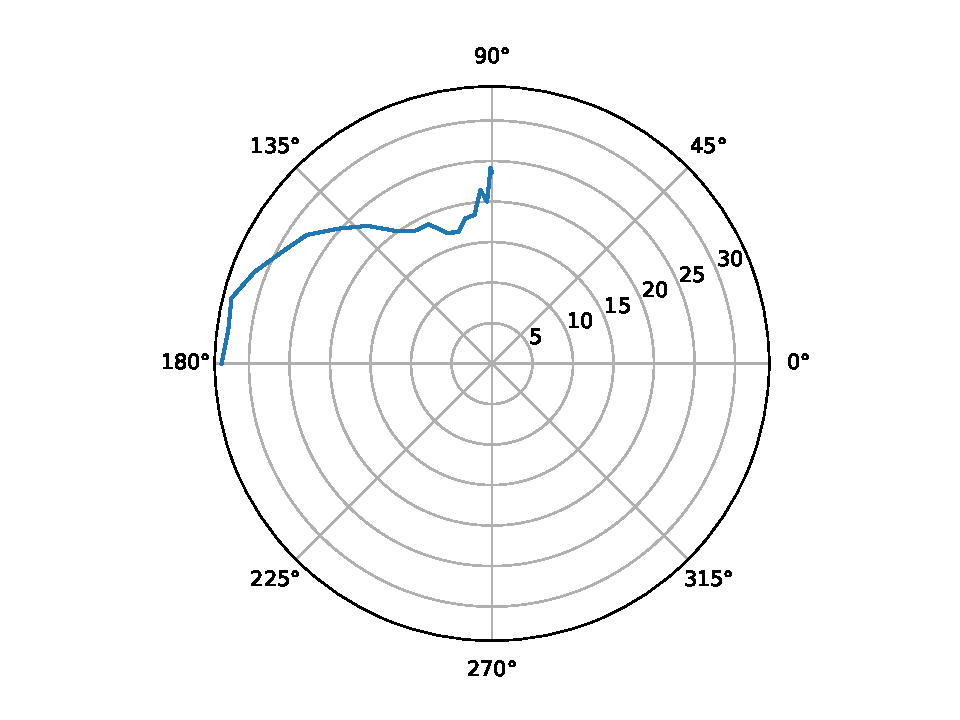
\includegraphics[scale=0.3]{./pictures/H_atom_resonanz_1_2310Hz.pdf}
                    \caption{In der Abbildung ist die Einhüllende, sowie das schwingende elektrische Feld eines linear gechirpten Laserpulses zu sehen.}
                    \label{fig:H_atom_resonanz_1_2310Hz}
                \end{subfigure}
                \hfill
                \centering
                \begin{subfigure}[b]{0.45\textwidth}
                    \centering
                    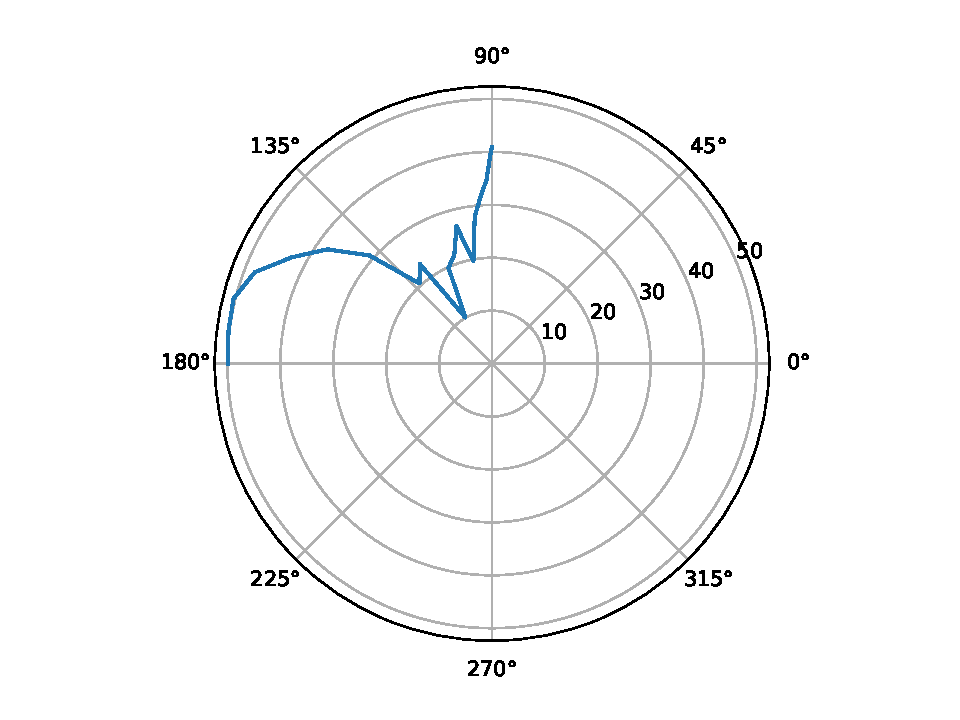
\includegraphics[scale=0.3]{./pictures/H_atom_resonanz_2_3711Hz.pdf}
                    \caption{In der Grafik wird der Chirp des Pulses als Änderung der Kreisfrequenz über den zeitlichen Verlauf des Pulses verdeutlicht.}
                    \label{fig:H_atom_resonanz_2_3711Hz}
                \end{subfigure}

                \centering
                \begin{subfigure}[b]{0.45\textwidth}
                    \centering
                    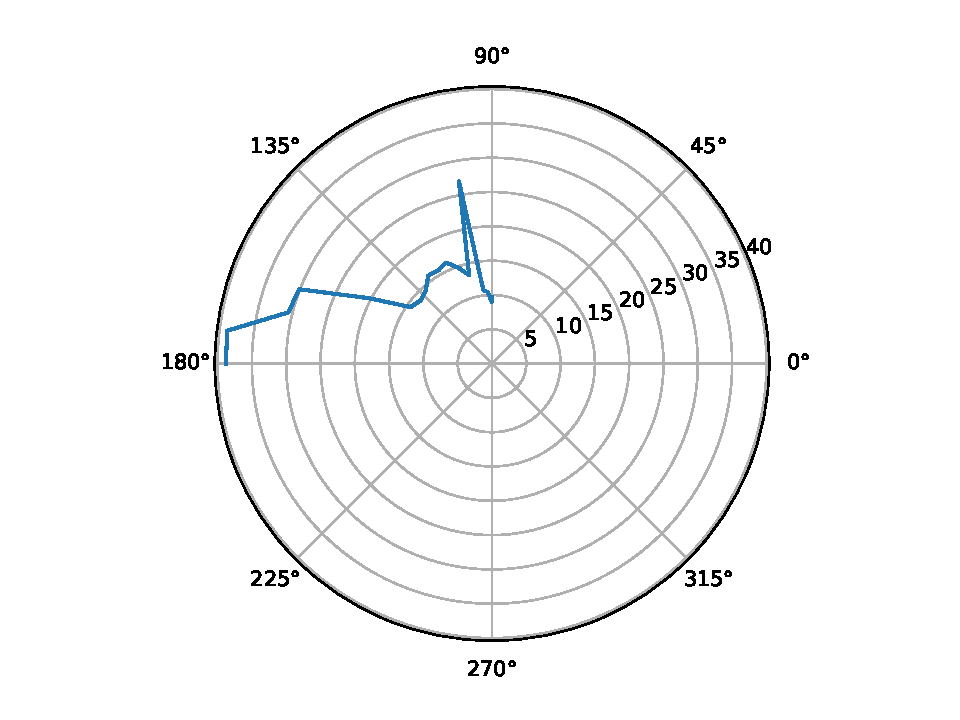
\includegraphics[scale=0.3]{./pictures/H_atom_resonanz_3_4999Hz.pdf}
                    \caption{In der Abbildung ist die Einhüllende, sowie das schwingende elektrische Feld eines linear gechirpten Laserpulses zu sehen.}
                    \label{fig:H_atom_resonanz_3_4999Hz}
                \end{subfigure}
                \hfill
                \centering
                \begin{subfigure}[b]{0.45\textwidth}
                    \centering
                    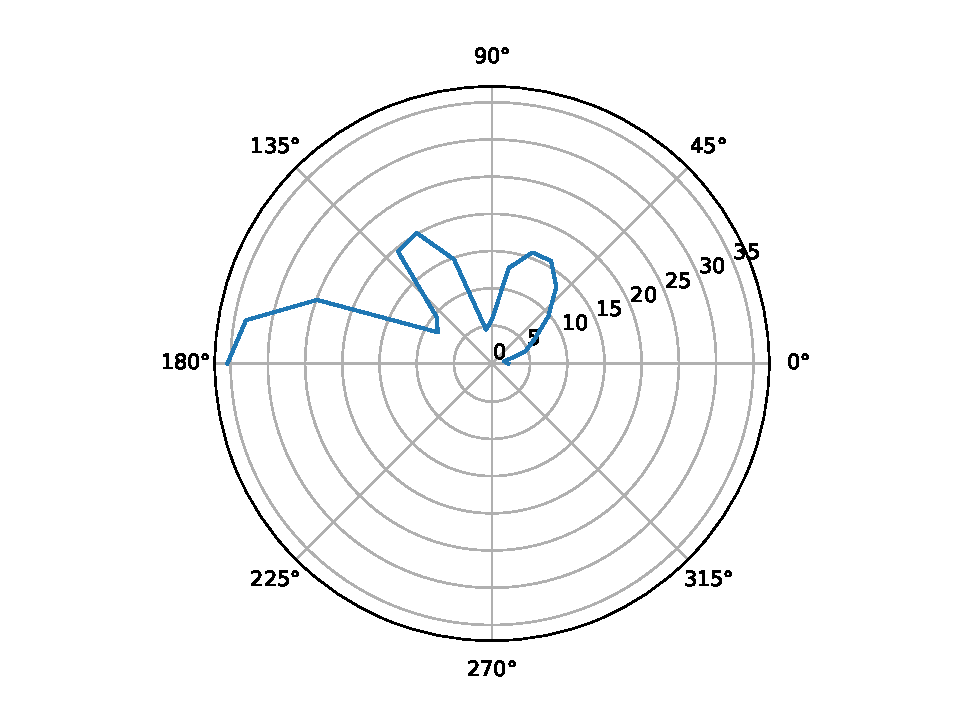
\includegraphics[scale=0.3]{./pictures/H_atom_resonanz_4_7470Hz.pdf}
                    \caption{In der Grafik wird der Chirp des Pulses als Änderung der Kreisfrequenz über den zeitlichen Verlauf des Pulses verdeutlicht.}
                    \label{fig:H_atom_resonanz_4_7470Hz}
                \end{subfigure}
            \end{figure}

        \FloatBarrier
        \newpage
        \subsubsection*{Zustandsaufspaltung}
            Nach dem Einsetzten von Zwischenringen ergeben sich Aufspaltungen der Resonanz um \SI{2.3}{\kilo\hertz}, die in Abbildung \ref{fig:hatom_180_3mm} exemplarisch für eine Ringlänge von 
            \SI{3}{\milli\metre} eingezeichnet ist.
            \FloatBarrier 
            \begin{figure}[ht]
                \centering
                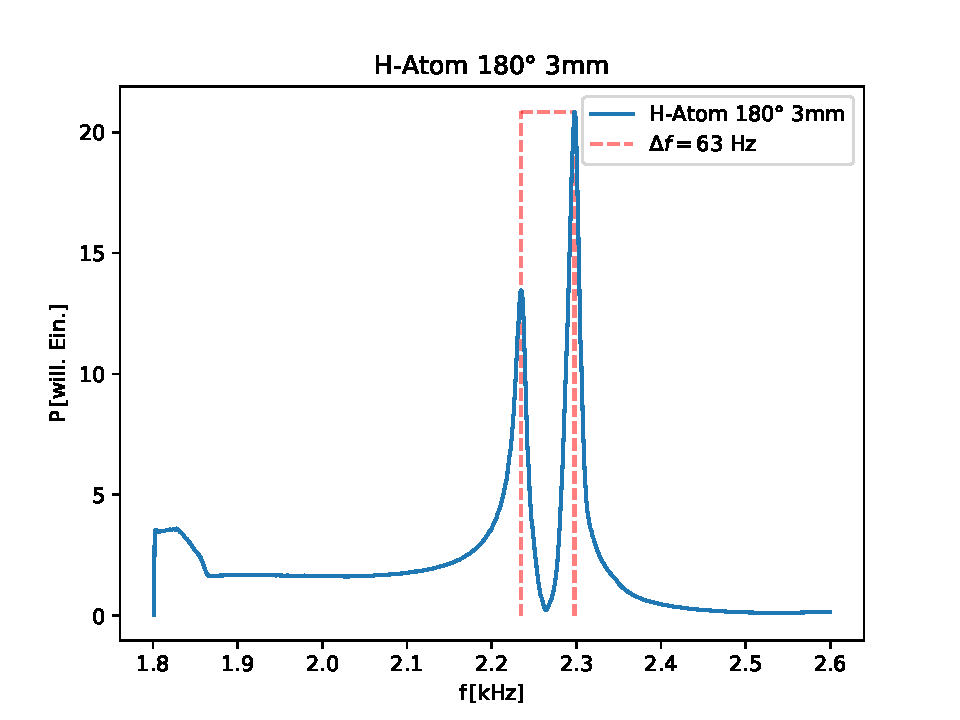
\includegraphics[scale=0.5]{./pictures/hatom_180_3mm.pdf}
                \caption{In der Abbildung ist die Einhüllende, sowie das schwingende elektrische Feld eines linear gechirpten Laserpulses zu sehen.}
                \label{fig:hatom_180_3mm}
            \end{figure}
            \FloatBarrier
            Die Aufspaltung der Resonanzfrequenzen steigt, wie in Abbildung~\ref{fig:f_Aufspaltung} zu sehen, mit linear mit der Länge des Zwischenrings auf einen maximalen Wert von \SI{171}{\hertz} an.
            Dies entspicht der zum Magnetfeld proportionalen Zeeman-Aufspaltung eines Wasserstoffatoms in einem externen Magnetfeld.
            \FloatBarrier
            \begin{figure}[ht]
                \centering
                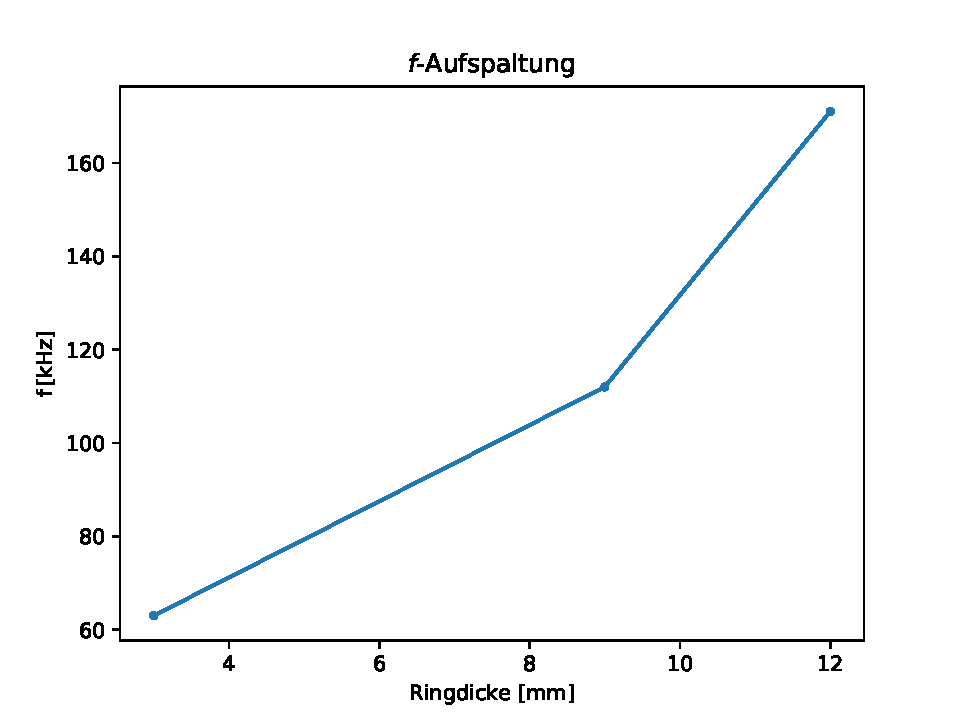
\includegraphics[scale=0.5]{./pictures/f_Aufspaltung.pdf}
                \caption{In der Abbildung ist die Einhüllende, sowie das schwingende elektrische Feld eines linear gechirpten Laserpulses zu sehen.}
                \label{fig:f_Aufspaltung}
            \end{figure}

        \subsubsection*{Winkelabhängigkeit der Zustandsaufspaltung}
            Die Winkelabhängigkeit der Druckamplitudenverteilungen ist für einen Zwischenring der Länge \SI{9}{\milli\metre} in einem Polarplot \ref{fig:H_atom_resonanz_4} aufgetragen.  
            \FloatBarrier 
            \begin{figure}[ht]
                \centering
                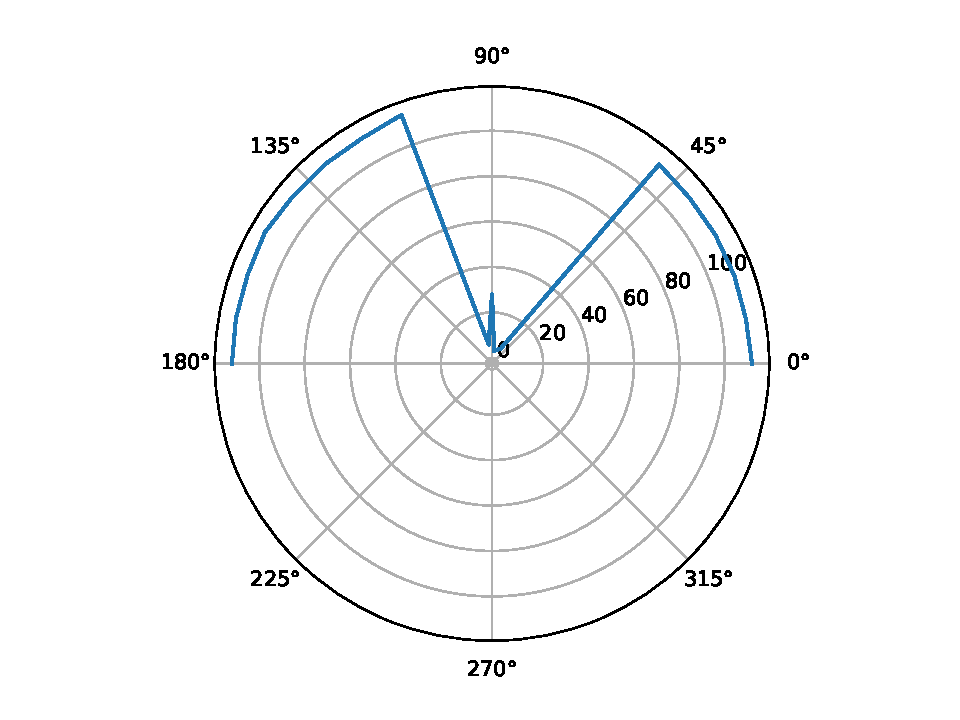
\includegraphics[scale=0.5]{./pictures/H_atom_resonanz_4.pdf}
                \caption{In der Abbildung ist die Einhüllende, sowie das schwingende elektrische Feld eines linear gechirpten Laserpulses zu sehen.}
                \label{fig:H_atom_resonanz_4}
            \end{figure}
            \FloatBarrier
            Die Aufspaltung ist Abbildung~\ref{fig:hatom_180_9mm} exemplarisch für einen Winkel von 180° dargestellt. Die Resonanzfrequenz bei \SI{2.170}{\kilo\hertz} entspricht einem Zustand mit den 
            Quantenzahlen m=0 und l=1 . Die Resonanzfrequenz bei \SI{2.284}{\kilo\hertz} entspricht dem Zustand mit den Quantenzahlen m=$\pm 1$ und l=1. Diese Aufspaltung ist wieder das Äquivalent des
            Zeeman-Effekts, der in diesem Fall der Änderung einer Symmetrieachse, durch das Verlängern des Resonators in eine Richtung entspricht.
            \FloatBarrier
            \begin{figure}[ht]
                \centering
                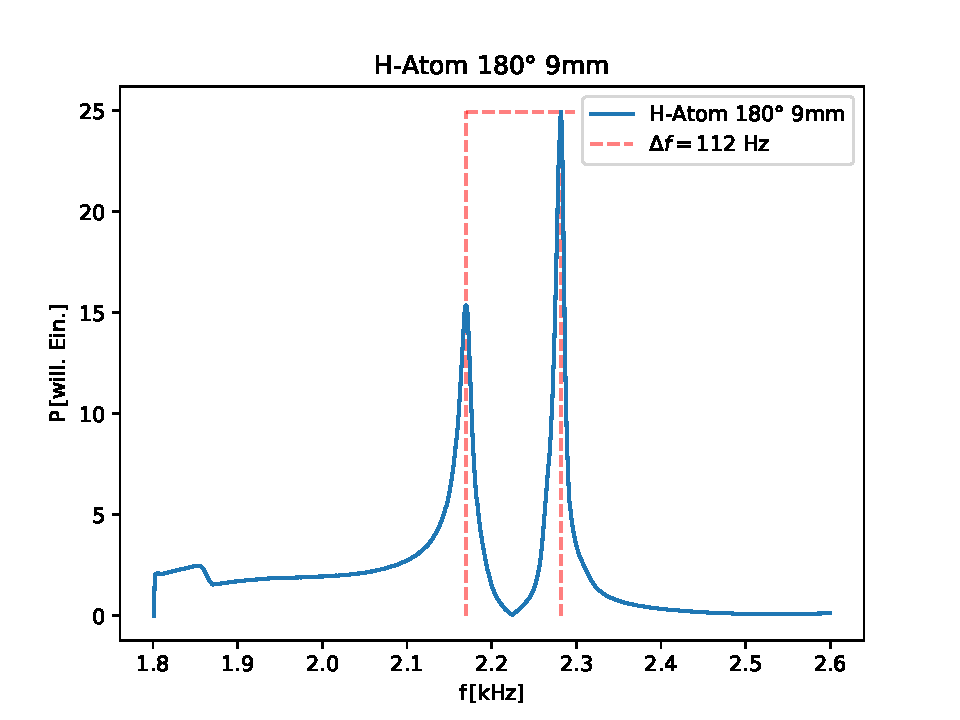
\includegraphics[scale=0.5]{./pictures/hatom_180_9mm.pdf}
                \caption{In der Abbildung ist die Einhüllende, sowie das schwingende elektrische Feld eines linear gechirpten Laserpulses zu sehen.}
                \label{fig:hatom_180_9mm}
            \end{figure}

    \subsection{Wasserstoffmolekül}
        \subsubsection*{Resonanzfrequenzen für verschiedene Blendendurchmesser}
            Für die verschiedenen Blendendurchmesser \SI{10}{\milli\metre}, \SI{15}{\milli\metre} und \SI{20}{\milli\metre} ergeben sich im Frequenzbereich von 2,2 bis \SI{2.5}{\kilo\hertz} drei 
            Resonanzfrequenzen, deren exakte Werte in Abhängigkeit vom Blendendurchmesser in Abbildung \ref{fig:res_freq_gegen_d_blende} aufgetragen sind. Es ist deutlich zu erkennen, dass nur die dritte
            Resonanzfrequenz vom Blendendurchmesser abhängt. 
            \begin{figure}[ht]
                \centering
                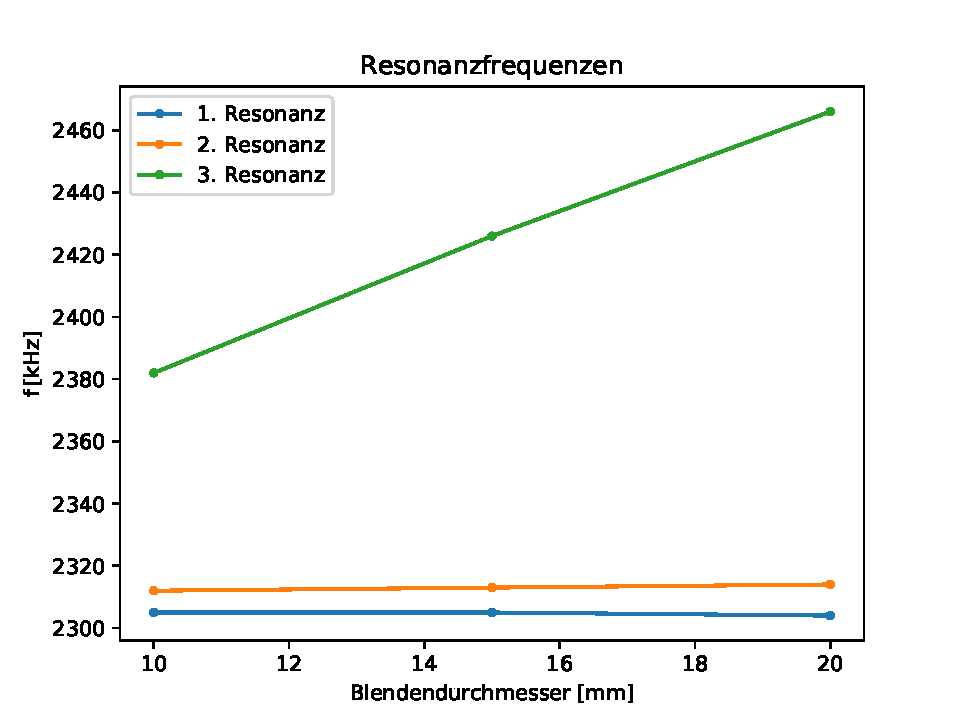
\includegraphics[scale=0.5]{./pictures/res_freq_gegen_d_blende.pdf}
                \caption{In der Abbildung ist die Einhüllende, sowie das schwingende elektrische Feld eines linear gechirpten Laserpulses zu sehen.}
                \label{fig:res_freq_gegen_d_blende}
            \end{figure}
        \FloatBarrier
        \subsubsection*{Winkelabhängigkeit gewählter Resonanzfrequenzen}
            Während für einen Blendendurchmesser von \SI{16}{\milli\metre} maximal vier Resonanzen zu erwarten sind, werden wie in Abbildung \ref{fig:hmol_res} zu sehen nur die Resonanzfrequenzen 
            \SI{2307}{\hertz}, \SI{2313}{\hertz} und \SI{2426}{\hertz} gemessen.  
            \begin{figure}[ht]
                \centering
                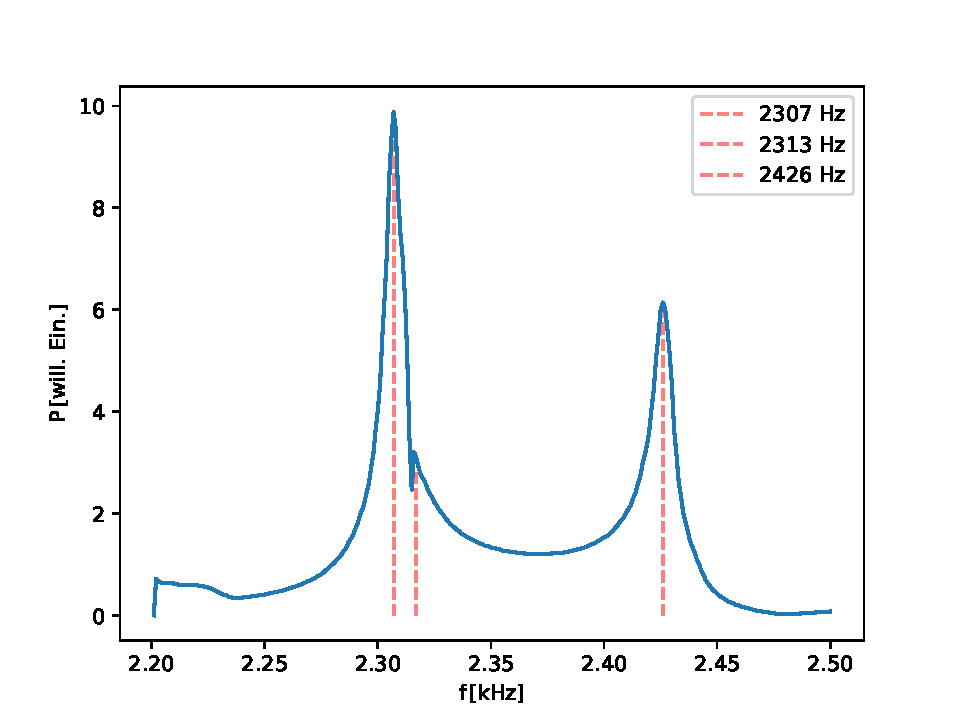
\includegraphics[scale=0.5]{./pictures/hmol_res.pdf}
                \caption{In der Abbildung ist die Einhüllende, sowie das schwingende elektrische Feld eines linear gechirpten Laserpulses zu sehen.}
                \label{fig:hmol_res}
            \end{figure}
            \FloatBarrier
            Für diese drei Resonanzfrequenzen werden die Druckamplituden in Abhängigkeit vom Winkel $\alpha$ in Polarplots aufgetragen 

            \FloatBarrier
            \begin{figure}[ht]
                \centering
                \begin{subfigure}[b]{0.45\textwidth}
                    \centering
                    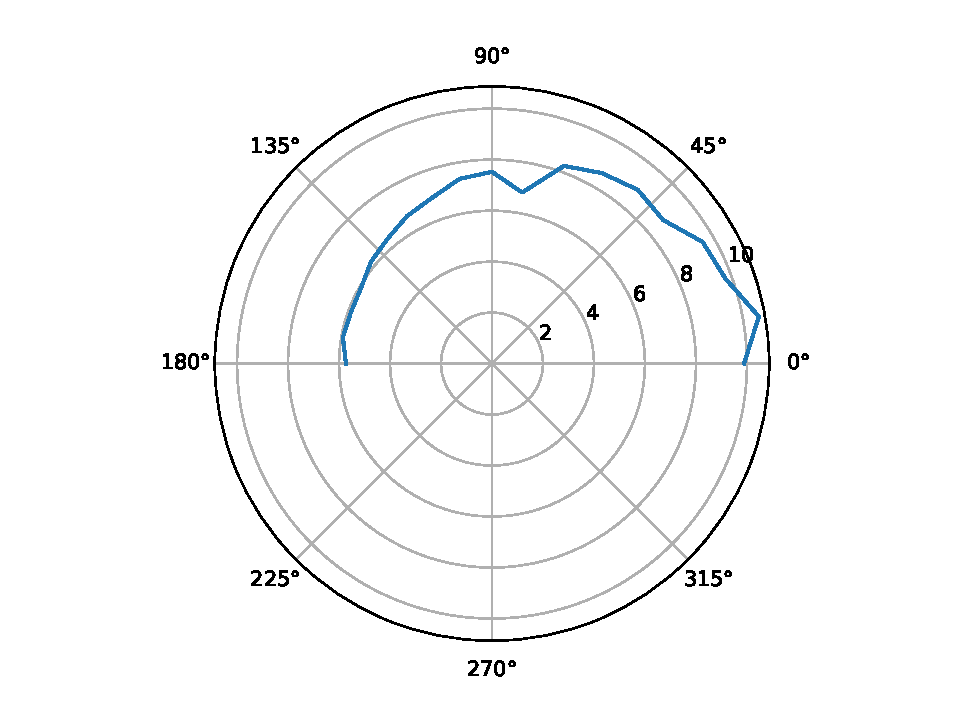
\includegraphics[scale=0.3]{./pictures/H_mol_resonanz_1_2307Hz.pdf}
                    \caption{In der Abbildung ist die Einhüllende, sowie das schwingende elektrische Feld eines linear gechirpten Laserpulses zu sehen.}
                    \label{fig:H_mol_resonanz_1_2307Hz}
                \end{subfigure}
                \hfill
                \centering
                \begin{subfigure}[b]{0.45\textwidth}
                    \centering
                    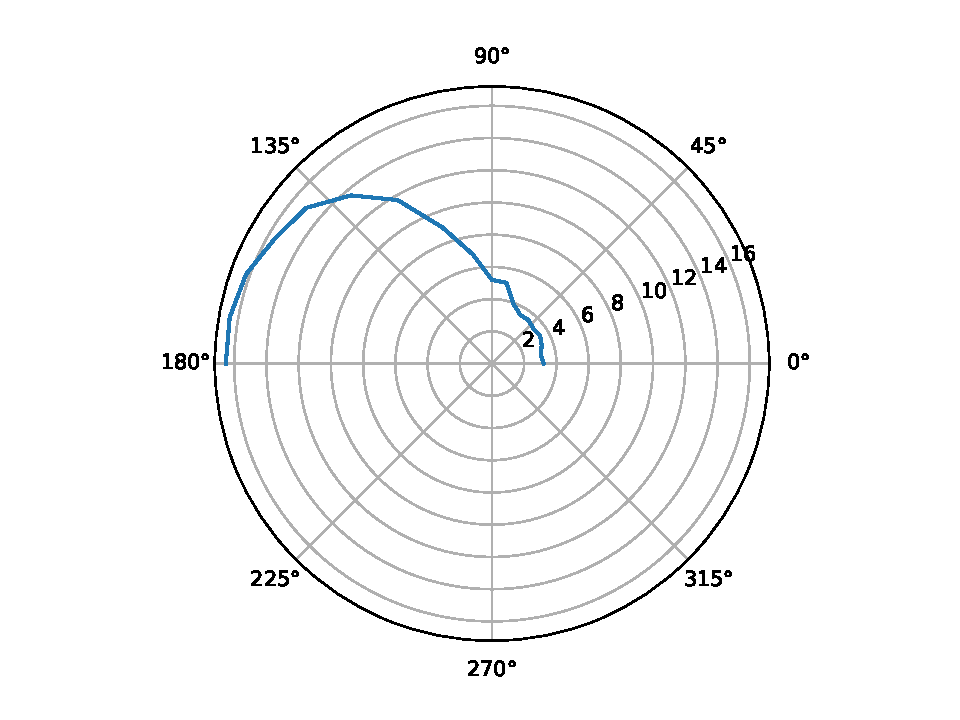
\includegraphics[scale=0.3]{./pictures/H_mol_resonanz_1_2313Hz.pdf}
                    \caption{In der Grafik wird der Chirp des Pulses als Änderung der Kreisfrequenz über den zeitlichen Verlauf des Pulses verdeutlicht.}
                    \label{fig:H_mol_resonanz_1_2313Hz}
                \end{subfigure}

                \centering
                \begin{subfigure}[b]{0.45\textwidth}
                    \centering
                    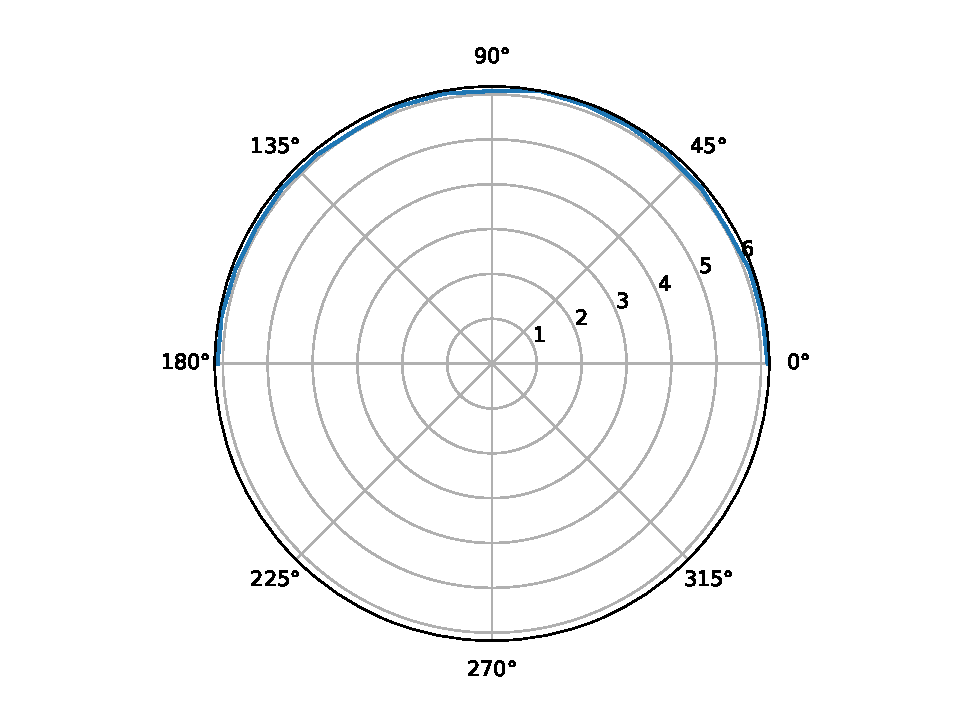
\includegraphics[scale=0.3]{./pictures/H_mol_resonanz_1_2426Hz.pdf}
                    \caption{In der Abbildung ist die Einhüllende, sowie das schwingende elektrische Feld eines linear gechirpten Laserpulses zu sehen.}
                    \label{fig:H_mol_resonanz_1_2426Hz}
                \end{subfigure}
            \end{figure}
            \FloatBarrier
            und die Phasenverschiebungen bei einem Winkel von 180° zwischen der Druckamplitude im oberen und unteren Teil des Resonators aufgelistet~\ref{tab:rel_phasenverschiebung}.
            \FloatBarrier
            \begin{table}[h]
                \centering
                \caption{In dieser Tabelle sind für die Ordnungen 1 bis 11 die Resonanzfrequenzen $f_{\text{res}}$, die zugehörigen Amplituden und Phasenverschiebungen $\varphi$.}
                \label{tab:rel_phasenverschiebung}
                \begin{tabular}{c c c c c}
                \toprule
                {Ordnung} & {$f_{\text{res}}$ [$\si{\kilo\hertz}]$} & {Phasendiff. oben [°]} & {Phasendiff. unten [°]} & {relative Phasendiff. [°]} \\
                \midrule
                \num{1}  & \num{2.307}  &  \num{-109}  &  \num{-36}   & \num{73}      \\
                \num{2}  & \num{2.313}  &  \num{-103}  &  \num{-85}   & \num{188}     \\
                \num{3}  & \num{2.426}  &  \num{36}    &  \num{-145}  & \num{181}     \\
                \bottomrule
                \end{tabular}
            \end{table}
            AuswertungstextAuswertungstextAuswertungstextAuswertungstextAuswertungstextAuswertungstextAuswertungstextAuswertungstextAuswertungstextAuswertungstextAuswertungstextAuswertungstextAuswert
            AuswertungstextAuswertungstextAuswertungstextAuswertungstextAuswertungstextAuswertungstextAuswertungstextAuswertungstextAuswertungstextAuswertungstextAuswertungstextAuswertungstextAuswert
            AuswertungstextAuswertungstextAuswertungstextAuswertungstextAuswertungstextAuswertungstextAuswertungstextAuswertungstextAuswertungstextAuswertungstextAuswertungstextAuswertungstextAuswert
            AuswertungstextAuswertungstextAuswertungstextAuswertungstextAuswertungstextAuswertungstextAuswertungstextAuswertungstextAuswertungstextAuswertungstextAuswertungstextAuswertungstextAuswert
            AuswertungstextAuswertungstextAuswertungstextAuswertungstextAuswertungstextAuswertungstextAuswertungstextAuswertungstextAuswertungstextAuswertungstextAuswertungstextAuswertungstextAuswert

    \subsection{Ein-Dimensionaler Festkörper}
        \subsubsection*{Resonatorkette mit 16mm-Blenden}
            Die aufgenommenen Frequenzspektren der Resonatorketten zeigen jeweils vier Bereiche, die mit Maxima gefüllt sind. Wie in den 
            Abbildungen~\ref{fig:1dim_2_Zylinder_16mm,fig:1dim_4_Zylinder_16mm,fig:1dim_10_Zylinder_16mm} zu erkennen, entspricht die Anzahl der Maxima der der verwendeten Zylinder. Dies lässt sich so 
            interpretieren, dass durch jeden Zylinder ein Band hinzugefügt wird, auf dem Elektronen in einem Festkörper Zustände einnehmen können. Die Bereiche ohne Maxima entsprechen Bandlücken, also Bereichen,
            in denen keine Elektronenzustände vorliegen.     
            
            \FloatBarrier
            \begin{figure}[ht]
                \centering
                \begin{subfigure}[b]{0.45\textwidth}
                    \centering
                    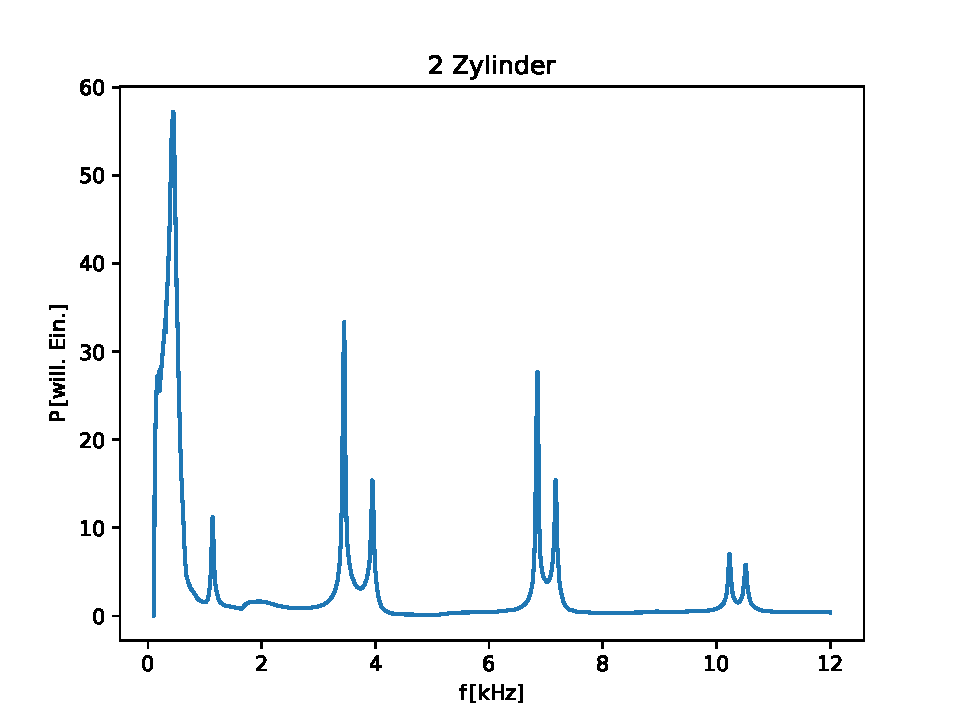
\includegraphics[scale=0.45]{./pictures/1dim_2_Zylinder_16mm.pdf}
                    \caption{In der Abbildung ist die Einhüllende, sowie das schwingende elektrische Feld eines linear gechirpten Laserpulses zu sehen.}
                    \label{fig:1dim_2_Zylinder_16mm}
                \end{subfigure}
                \hfill
                \centering
                \begin{subfigure}[b]{0.45\textwidth}
                    \centering
                    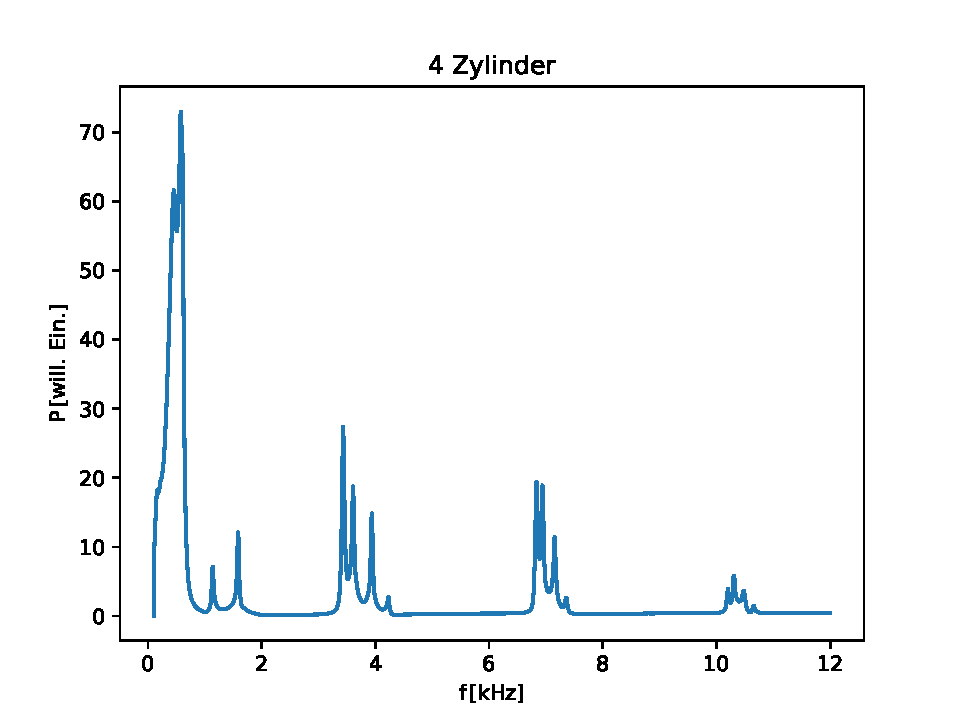
\includegraphics[scale=0.45]{./pictures/1dim_4_Zylinder_16mm.pdf}
                    \caption{In der Grafik wird der Chirp des Pulses als Änderung der Kreisfrequenz über den zeitlichen Verlauf des Pulses verdeutlicht.}
                    \label{fig:1dim_4_Zylinder_16mm}
                \end{subfigure}

                \centering
                \begin{subfigure}[b]{0.45\textwidth}
                    \centering
                    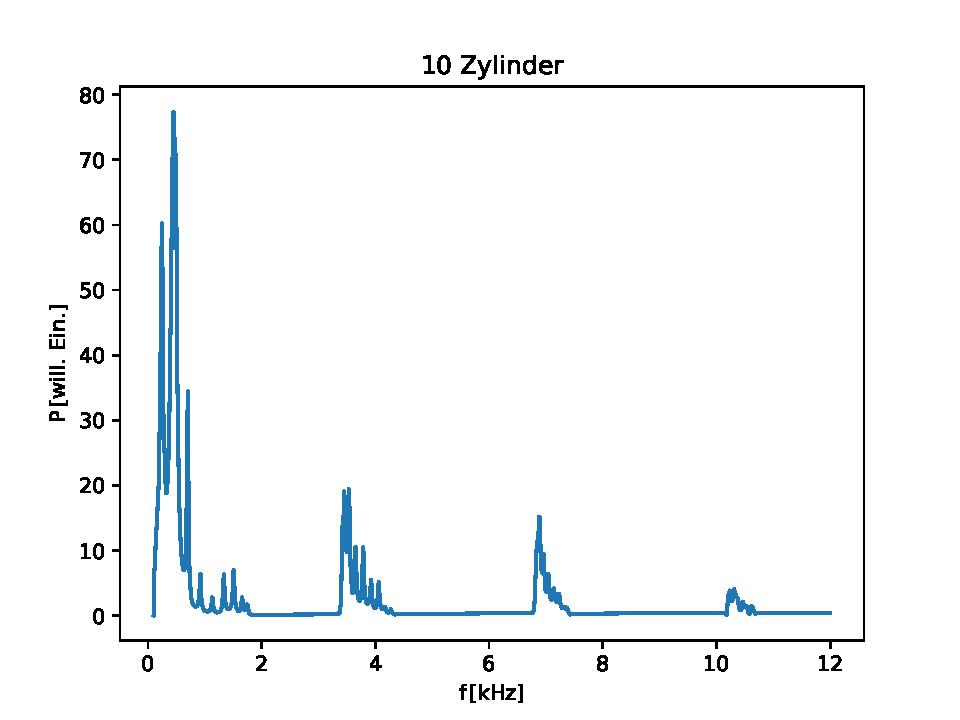
\includegraphics[scale=0.45]{./pictures/1dim_10_Zylinder_16mm.pdf}
                    \caption{In der Abbildung ist die Einhüllende, sowie das schwingende elektrische Feld eines linear gechirpten Laserpulses zu sehen.}
                    \label{fig:1dim_10_Zylinder_16mm}
                \end{subfigure}
            \end{figure}
            \FloatBarrier


        \subsubsection*{Resonatorkette mit 10mm- und 13mm-Blenden}
            Ein kleinerer Blendendurchmesser entspricht einem größeren Potential innerhalb des Festkörpers. Demnach sind die Elektronen stärker lokalisiert und ihre Bänder flacher. Dies ist in den 
            Abbildungen~\ref{10mm_16mm_blende} zu erkennen. Besonders für die Frequenzspektren bei einer Blendenwahl von \SI{10}{\milli\metre} sind die kleineren Abstände zwischen den Maxima und die größeren
            Abstände zwischen den Maximabereichen im Vergleich zu den Frequenzspektren bei einer Blendenwahl von \SI{16}{\milli\metre} deutlich zu erkennen.
            \FloatBarrier
            \begin{figure}[ht]
                \centering
                \begin{subfigure}[b]{0.45\textwidth}
                    \centering
                    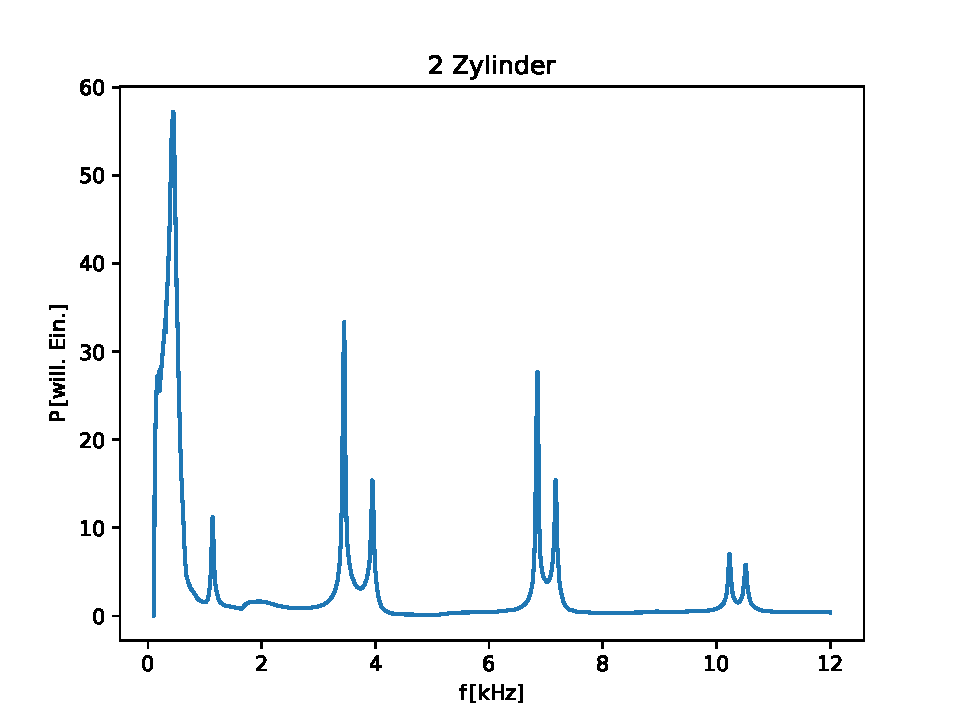
\includegraphics[scale=0.45]{./pictures/1dim_2_Zylinder_10mm.pdf}
                    \caption{In der Abbildung ist die Einhüllende, sowie das schwingende elektrische Feld eines linear gechirpten Laserpulses zu sehen.}
                    \label{fig:1dim_2_Zylinder_10mm}
                \end{subfigure}
                %\hfill
                \centering
                \begin{subfigure}[b]{0.45\textwidth}
                    \centering
                    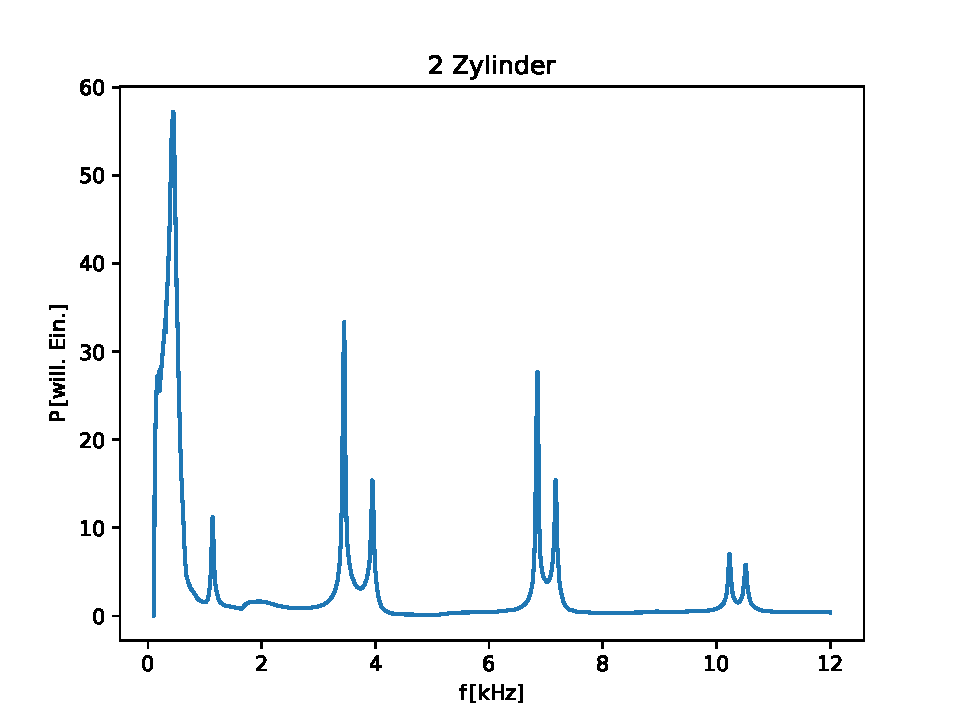
\includegraphics[scale=0.45]{./pictures/1dim_2_Zylinder_13mm.pdf}
                    \caption{In der Grafik wird der Chirp des Pulses als Änderung der Kreisfrequenz über den zeitlichen Verlauf des Pulses verdeutlicht.}
                    \label{fig:1dim_2_Zylinder_13mm}
                \end{subfigure}
                %\hfill
                \centering
                \begin{subfigure}[b]{0.45\textwidth}
                    \centering
                    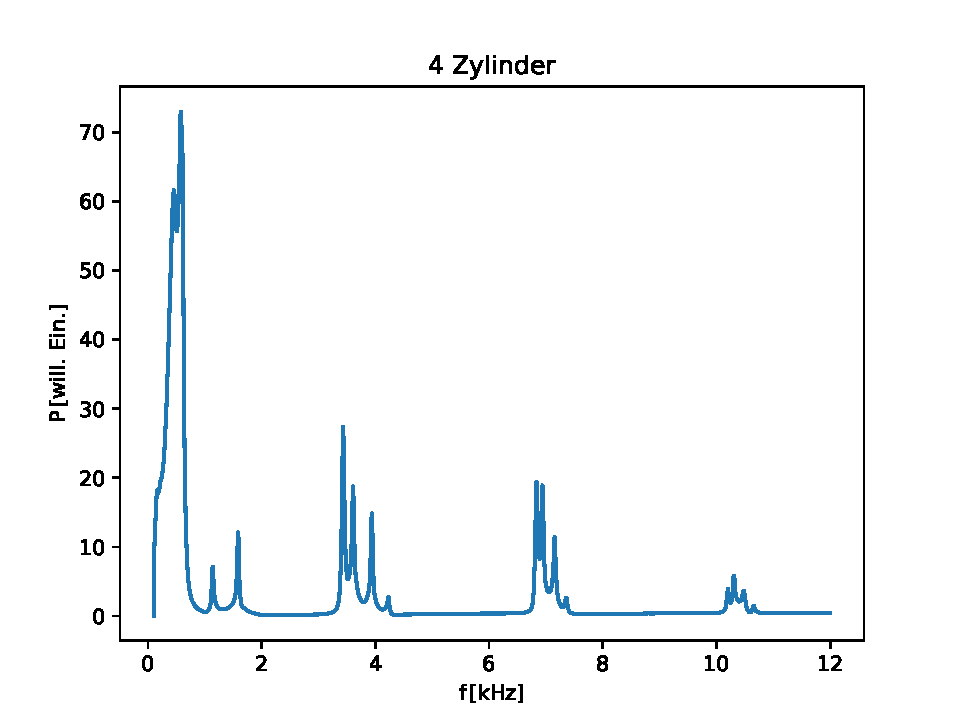
\includegraphics[scale=0.45]{./pictures/1dim_4_Zylinder_10mm.pdf}
                    \caption{In der Abbildung ist die Einhüllende, sowie das schwingende elektrische Feld eines linear gechirpten Laserpulses zu sehen.}
                    \label{fig:1dim_4_Zylinder_10mm}
                \end{subfigure}
                \centering
                \begin{subfigure}[b]{0.45\textwidth}
                    \centering
                    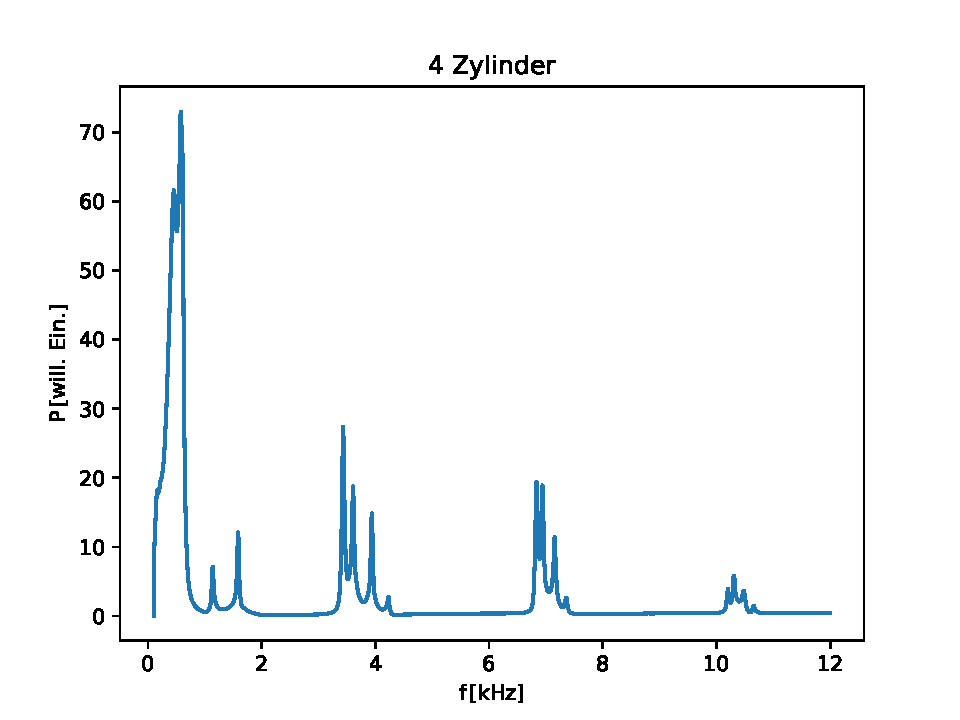
\includegraphics[scale=0.45]{./pictures/1dim_4_Zylinder_13mm.pdf}
                    \caption{In der Abbildung ist die Einhüllende, sowie das schwingende elektrische Feld eines linear gechirpten Laserpulses zu sehen.}
                    \label{fig:1dim_4_Zylinder_13mm}
                \end{subfigure}
                %\hfill
                \centering
                \begin{subfigure}[b]{0.45\textwidth}
                    \centering
                    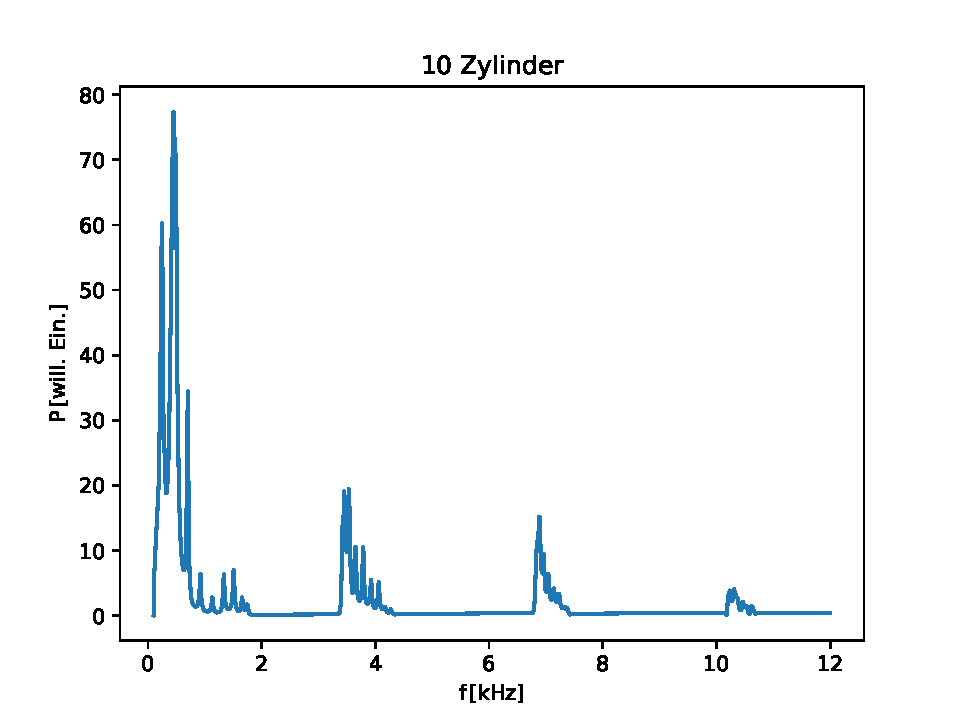
\includegraphics[scale=0.45]{./pictures/1dim_10_Zylinder_10mm.pdf}
                    \caption{In der Grafik wird der Chirp des Pulses als Änderung der Kreisfrequenz über den zeitlichen Verlauf des Pulses verdeutlicht.}
                    \label{fig:1dim_10_Zylinder_10mm}
                \end{subfigure}
                %\hfill
                \centering
                \begin{subfigure}[b]{0.45\textwidth}
                    \centering
                    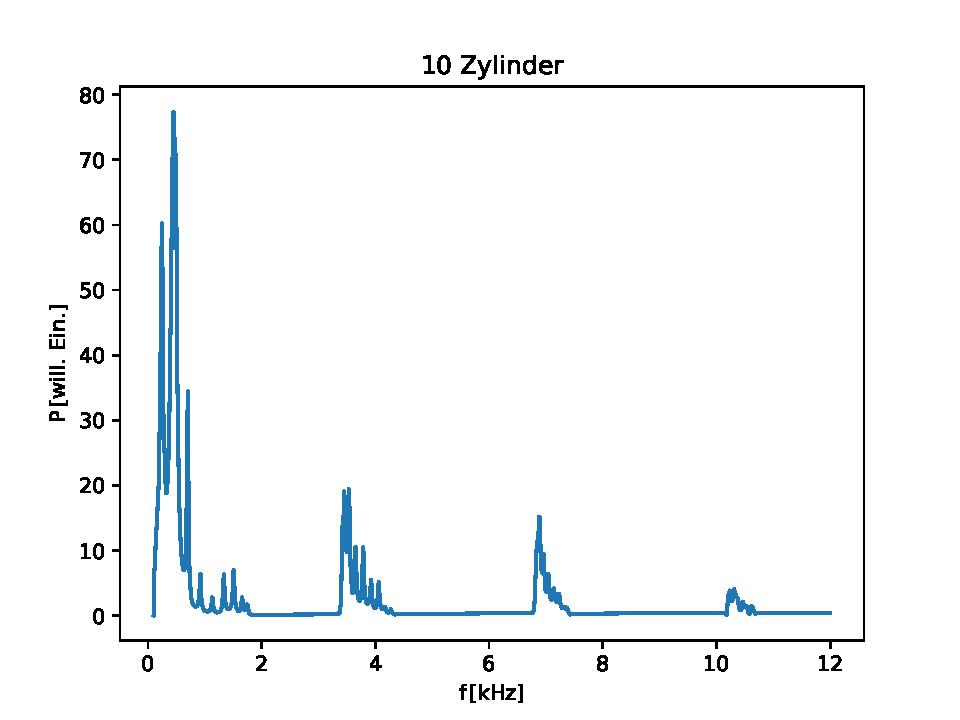
\includegraphics[scale=0.45]{./pictures/1dim_10_Zylinder_13mm.pdf}
                    \caption{In der Abbildung ist die Einhüllende, sowie das schwingende elektrische Feld eines linear gechirpten Laserpulses zu sehen.}
                    \label{fig:1dim_10_Zylinder_13mm}
                \end{subfigure}
                \caption{Auf der linken Seite sind die gemessenen Frequenzspektren für einen Blendendurchmesser von \SI{10}{\milli\metre} und die Zylinderanzahlen zwei, vier und 10 dargestellt. Auf der rechten Seite sind die entsprechenden Frequenzspektren für einen Blendendurchmesser von \SI{13}{\milli\metre} dargestellt.}
                \label{10mm_16mm_blende}
            \end{figure}
            \FloatBarrier


        \subsubsection*{Resonatorkette mit Störstellen}
            In Form von Zylindern abweichender Größe werden Störstellen erzeugt, die Gitterdefekten in Festkörpern entspechen simulieren sollen. Diese Störstellen rufen Abweichungen vom ungestörten 
            Frequenzspektrum hervor. So lässt sich für die Störzylinder der Größen \SI{62.5}{\milli\metre} (siehe Abb.~\ref{fig:1dim_4_Zylinder_625_Fehlstelle}) und 
            \SI{75}{\milli\metre}~\ref{fig:1dim_10_Zylinder_750_Fehlstelle} eine neue Resonanz um eine Frequenz von \SI{3}{\kilo\hertz} erkennen. Zudem ist, wie in Abbildung~\ref{fig:Störstelle} zu sehen, für 
            alle Störzylinder eine deutliche Reduktion der Druckamplituden im Vergleich zur ungestörten Resonatorkette aus zehen Zylindern zu erkennen. Auch ein Absacken der Druckamplituden in der Mitte des 
            ersten Maximabereichs zwischen 0 und \SI{3}{\kilo\hertz} ist für alle Störzylinderlängen gut zu erkennen.
            \FloatBarrier
            \begin{figure}[ht]
                \centering
                \begin{subfigure}[b]{0.45\textwidth}
                    \centering
                    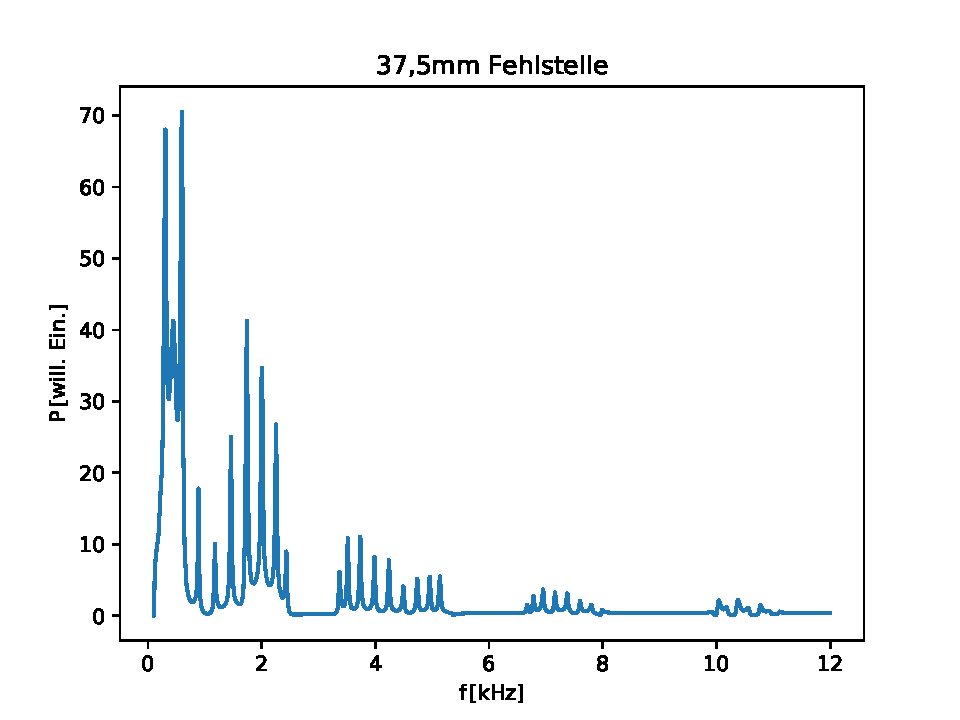
\includegraphics[scale=0.45]{./pictures/1dim_10_Zylinder_375_Fehlstelle.pdf}
                    \caption{In der Abbildung ist die Einhüllende, sowie das schwingende elektrische Feld eines linear gechirpten Laserpulses zu sehen.}
                    \label{fig:1dim_10_Zylinder_375_Fehlstelle}
                \end{subfigure}
                \hfill
                \centering
                \begin{subfigure}[b]{0.45\textwidth}
                    \centering
                    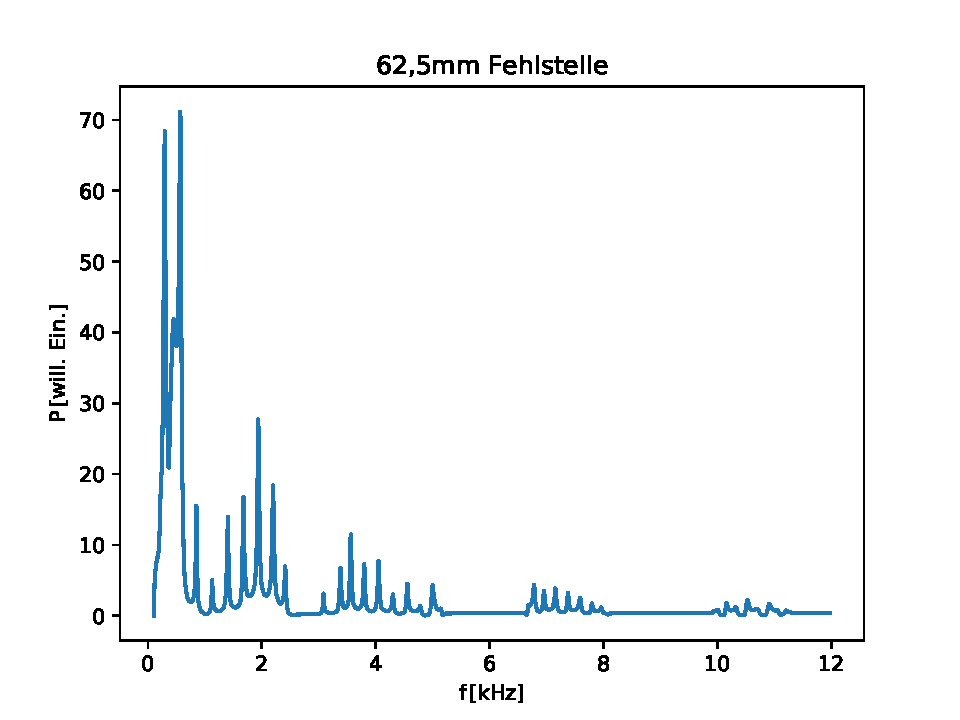
\includegraphics[scale=0.45]{./pictures/1dim_4_Zylinder_625_Fehlstelle.pdf}
                    \caption{In der Grafik wird der Chirp des Pulses als Änderung der Kreisfrequenz über den zeitlichen Verlauf des Pulses verdeutlicht.}
                    \label{fig:1dim_4_Zylinder_625_Fehlstelle}
                \end{subfigure}
                \centering
                \begin{subfigure}[b]{0.45\textwidth}
                    \centering
                    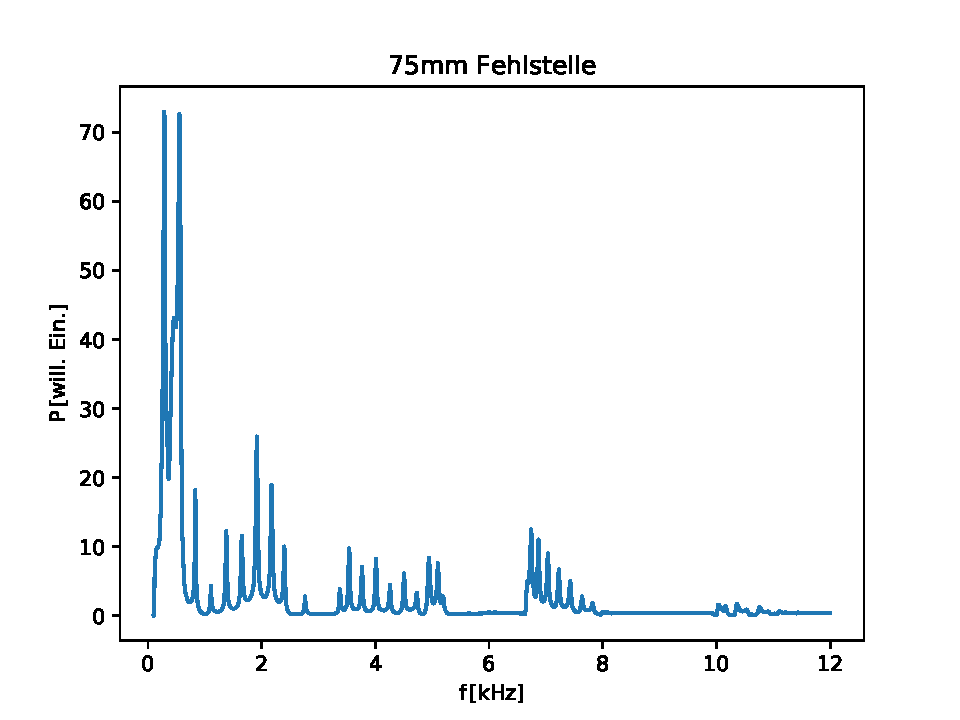
\includegraphics[scale=0.45]{./pictures/1dim_10_Zylinder_750_Fehlstelle.pdf}
                    \caption{In der Abbildung ist die Einhüllende, sowie das schwingende elektrische Feld eines linear gechirpten Laserpulses zu sehen.}
                    \label{fig:1dim_10_Zylinder_750_Fehlstelle}
                \end{subfigure}
                \caption{ }
                \label{fig:Störstelle}
            \end{figure}
            \FloatBarrier

        \subsubsection*{Kette wechselnder Resonatorlängen}
            Die Kette aus abwechselnden 50 und \SI{75}{\milli\metre} langen Resonatoren entspricht einem Gitter mit zwei-atomiger Basis. Dies führt dazu, dass die Resonanzen der einzelnen ein-atomigen Basen
            in die zwei-atomigen Basis  übernommen werden. Dies ist im Vergleich der einzelnen Spektren eines \SI{50}{\milli\metre}-Resonators (siehe Abb.~\ref{fig:1_Zylinder_50mm}) und eines 
            \SI{75}{\milli\metre}-Resonators (siehe Abb.~\ref{fig:1_Zylinder_75mm}) mit dem Spektrum der Kette wechselnder Resonatorlänge in Abbildung~\ref{fig:1dim_10_Zylinder_wechselnd_50_75} zu erkennen.
            \FloatBarrier
            \begin{figure}[ht]
                \centering
                \begin{subfigure}[b]{0.45\textwidth}
                    \centering
                    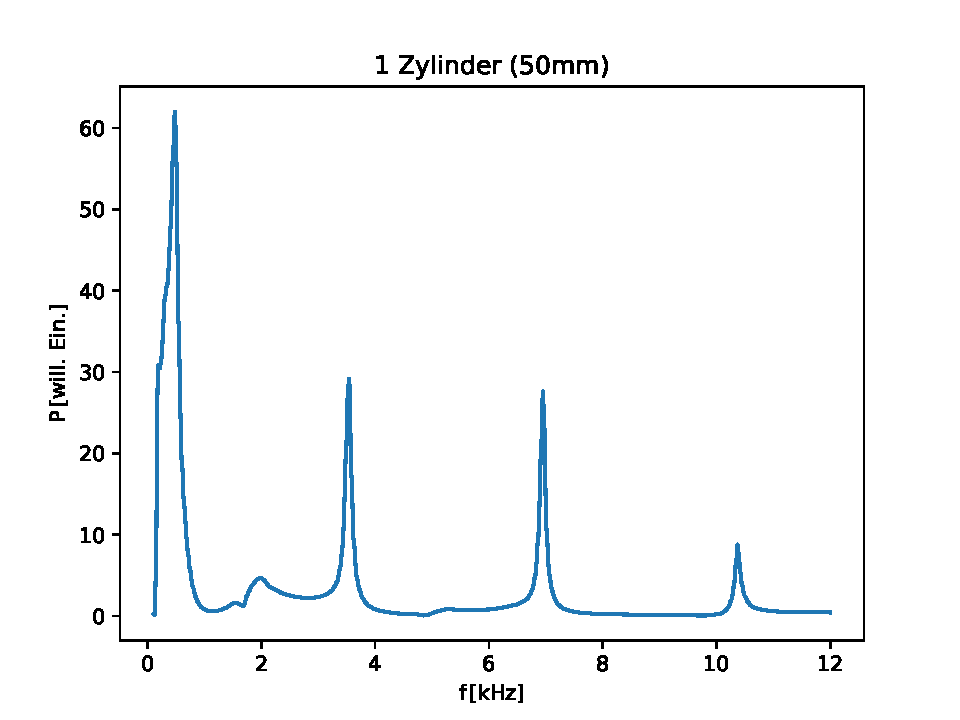
\includegraphics[scale=0.45]{./pictures/1_Zylinder_50mm.pdf}
                    \caption{In der Grafik wird der Chirp des Pulses als Änderung der Kreisfrequenz über den zeitlichen Verlauf des Pulses verdeutlicht.}
                    \label{fig:1_Zylinder_50mm}
                \end{subfigure}
                \hfill
                \centering
                \begin{subfigure}[b]{0.45\textwidth}
                    \centering
                    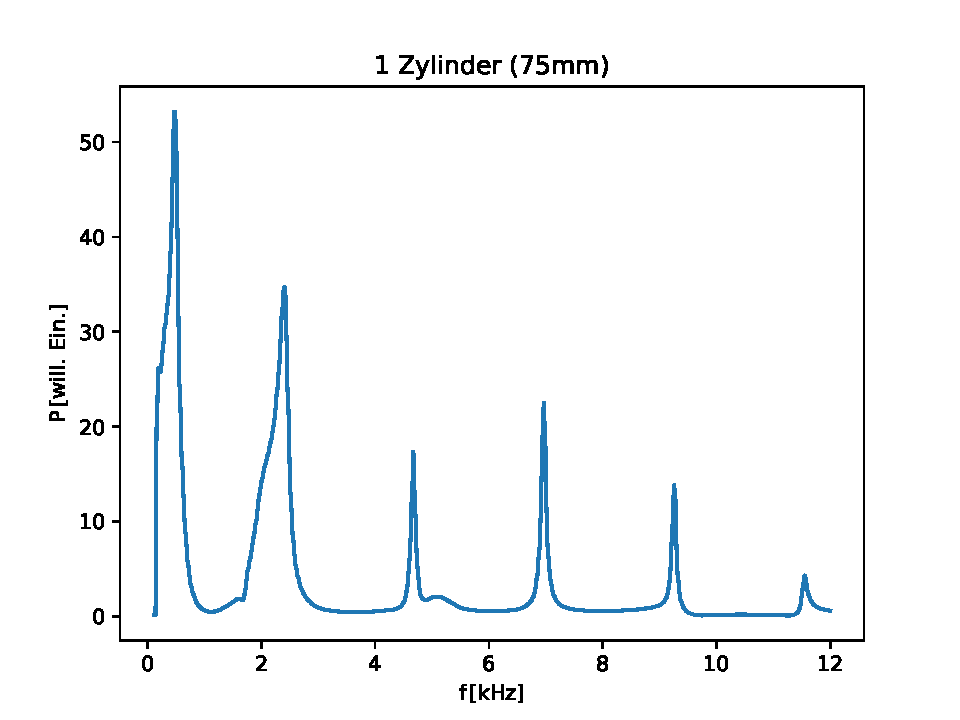
\includegraphics[scale=0.45]{./pictures/1_Zylinder_75mm.pdf}
                    \caption{In der Abbildung ist die Einhüllende, sowie das schwingende elektrische Feld eines linear gechirpten Laserpulses zu sehen.}
                    \label{fig:1_Zylinder_75mm}
                \end{subfigure}
                \centering
                \begin{subfigure}[b]{0.45\textwidth}
                    \centering
                    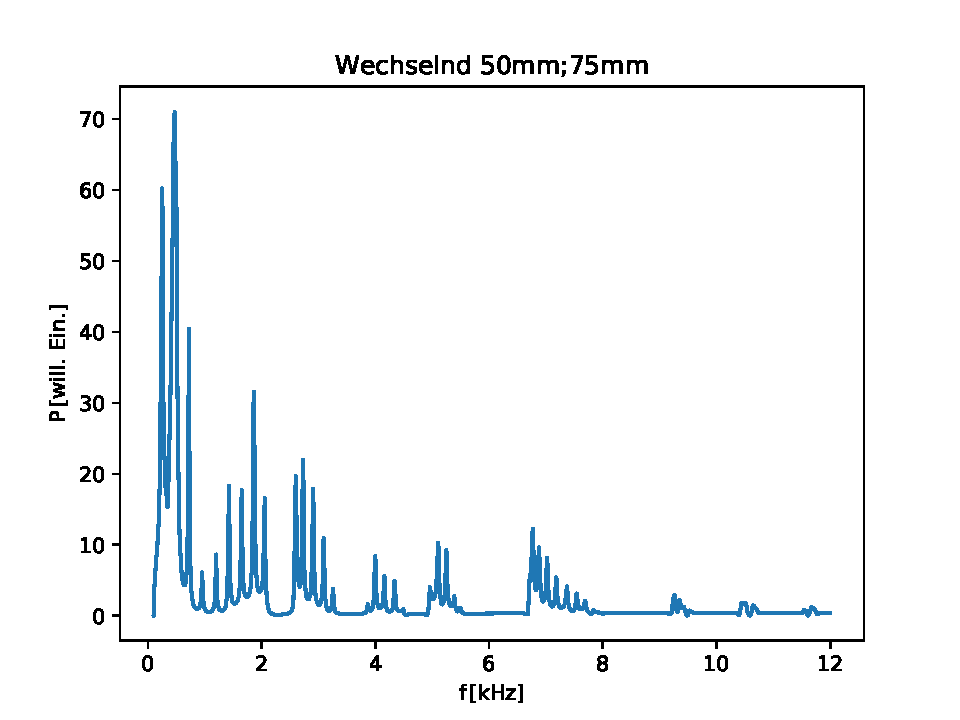
\includegraphics[scale=0.45]{./pictures/1dim_10_Zylinder_wechselnd_50_75.pdf}
                    \caption{In der Abbildung ist die Einhüllende, sowie das schwingende elektrische Feld eines linear gechirpten Laserpulses zu sehen.}
                    \label{fig:1dim_10_Zylinder_wechselnd_50_75}
                \end{subfigure}
                \caption{ }
                \label{fig:Wechselabbildung}
            \end{figure}
            \FloatBarrier
            
        \subsubsection*{Kette wechselnder Blendendurchmesser}
            Das bei wechselndem Blendendruchmesser von 13 und \SI{16}{\milli\metre} aufgenommene Frequenzspektrum ist in Abbildung~\ref{fig:1dim_8_Zylinder_blendewechselnd_13_16} dargestellt und zeigt eine 
            deutliche Aufspaltung der Maximabereiche um mindestens \SI{300}{\hertz}. Die neuen Bandlücken entstehen dadurch, dass sich das Potential nun alle zwei Zylinder periodisch wiederholt und nicht jeden 
            Zylinder. Dies entspricht einer neuen übergeordneten Periodizität des Gitters.  
            \begin{figure}[ht]
                \centering
                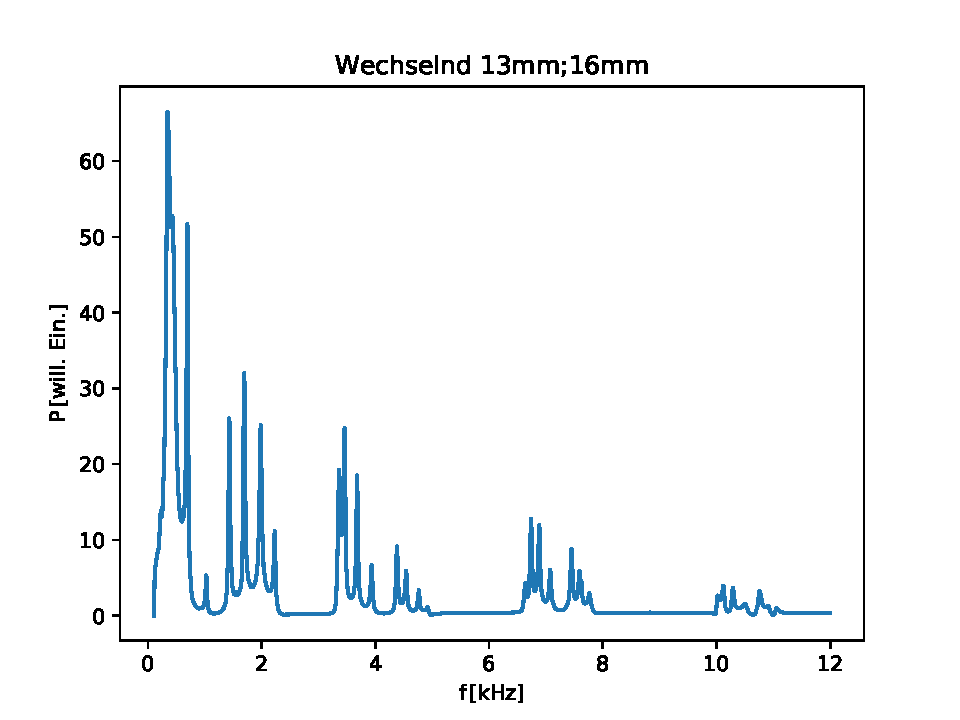
\includegraphics[scale=0.5]{./pictures/1dim_8_Zylinder_blendewechselnd_13_16.pdf}
                \caption{In der Abbildung ist die Einhüllende, sowie das schwingende elektrische Feld eines linear gechirpten Laserpulses zu sehen.}
                \label{fig:1dim_8_Zylinder_blendewechselnd_13_16}
            \end{figure}
            
            











































